
%\setcode{utf8}

\section{Kiwix Android Apps}
\label{section-kiwix-case-study}
Relying on analytics and reports provided by the Google Android's platform and presented in Google Play Console, we were able to reduce the crash rates of a family of Android apps. 
%
We chose the most sophisticated and complex of the Android apps, which also had the highest Crash rate at the time (see Table~\ref{tab:gpc_kiwix_apps_11_feb_2019}). The reduction went from over 5\% to under 0.25\% during the case study.

Figure~\ref{fig:android-vitals-kiwix-android-crash-rate-vs-peers} provides an illustrative example of the crash rate for Kiwix Android. The comparison with its peers, apps in the same category across Google Play, also shows Kiwix Android was in the bottom 7\% in terms of crash rate in that category. So the app was unreliable by either measure.

By applying what the team learned about crashes reported in Android Vitals the team was able to reduce the crash rate of this app several fold. When the improved codebase was used to refresh various custom apps their crash rates also decreased several fold.

\begin{figure}
    \centering
    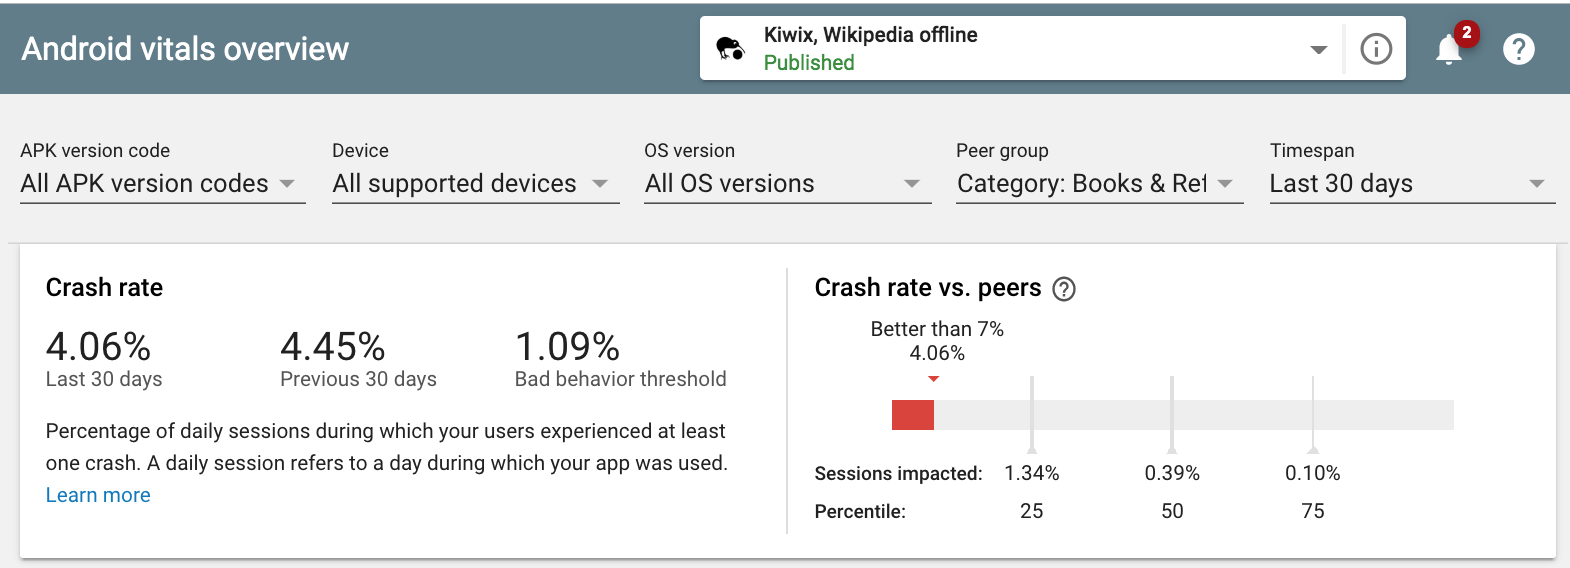
\includegraphics[width=13cm]{images/android-vitals-screenshots/Example-crash-rate-vs-peers 10-jun-2019.png}
    \caption{Android Vitals Kiwix Android crash rate vs peers \nth{10} June 2019}
    \label{fig:android-vitals-kiwix-android-crash-rate-vs-peers}
\end{figure}

Note: I have been involved in various aspects of Kiwix since 2014 including helping with the Android app, with manual and automated testing, with the PHeT project mentioned here, and so on.

\setminted{fontsize=\small,baselinestretch=1}

\subsection*{Evidence}
  \begin{minted}[
    gobble=4,
    frame=single,
    fontsize=\tiny,
    breaklines=true
  ]{yaml}
    evidence available :
      vitals-scraper : ~/sandbox/vitals-scraper-logs/android-stability-analysis/data/from-android-vitals
      google-play-console-reports : ~/Dropbox/Google Play Console Reports/reports/catrobat/pocketcode/crashes
      various-materials : in Dropbox
      co-written-paper : MOBILESoft 2019~\citep{harty_google_play_console_insightful_development_using_android_vitals_and_pre_launch_reports}, WAMA 2019~\citep{harty_better_android_apps_using_android_vitals}, MOBILESoft 2020~\citep{harty_improving_app_quality_despite_flawed_mobile_analytics}, ICST 2020~\citep{harty2020_how_can_software_testing_be_improved_by_analytics_to_deliver_better_apps}.
    evidence-needed : 
      Supporting materials for Phase 2:
      Supporting materials for Phase 3: 
      Releases and their release dates.
      Latest status of the tickets related  to crashes and ANRs.
      Current stability metrics for the Kiwix apps.
  \end{minted}

\subsection{Introduction of Kiwix Android Case Study}
%Introduce Kiwix at the risk of repetition. 
% TODO replace URLs with citations.
Kiwix makes knowledge available to people with no or limited internet access (\emph{i.e.} four billion people) by providing highly compressed content and a reader for the bespoke compression format. Anyone is free to use the software and the content. The project includes an offline reader for online content like Wikipedia, Project Gutenberg, or TED Talks and the project also develops and maintains software to download, compress, package, and make content easy to download and share~\citep{kiwix_about_the_project, gomez2017_wikimedia_kiwix_article}.

The project provides offline access to Wikipedia materials and many other read-only materials including TED talks, StackExchange sites, interactive science simulations, and others~\citep{kiwix_about_the_project, gomez2017_wikimedia_kiwix_article}. The project team has a long history of gathering for multi-day immersive hackathons~\footnote{e.g. \url{https://wiki.kiwix.org/wiki/Hackathons} and the researcher participated in several of these before this case study, the subsequent planned hackathons was canceled because of Covid-19.}

The Android project comprises various apps all based on a common opensource codebase. The core case study captures activities from early 2019 to early 2020; however the project is a long-term, ongoing project and I am still involved with it. Several post case-study updates will be covered in later chapters. The crash rate had been excessive for over a year and far exceeded the bad behaviour threshold Google Play specified. 

The case study started with a period of observation and discussion of the crash rate in particular as it had increased repeatedly and to such an extent that the 2.3 release had been aborted by the project team, various details follow.

In mid-April 2018 the reported crash rate was 1.53\%~\footnote{Details available in \href{https://github.com/kiwix/kiwix-android/issues/712}{issue 712} for the Kiwix Android project, the main app releases were version 2.2 and 2.3 at the time.}. By mid-June 2018 the overall crash rate had increased to 1.71\%~\footnote{The crash rate for version 2.2 was 2.03\% in the 30 days to \nth{14} June 2018.}. The rollout for 2.3 was aborted in February 2019~\footnote{The milestone for this release and the issues that were addressed is available online~\url{https://github.com/kiwix/kiwix-android/milestone/1?closed=1}.} as there was a crash that affected 10\% to 20\% of the users (according to the lead developer at the time). The crash rate for the app averaged over 5\% in January and February 2019. 


%\akb{Provide dates over which the excessive crash rate was noted? Also, while the project is a long-term, ongoing project, your case study captures its activity during a specific window.}

The project team actively exclude any tracking or analytics within the app to minimise the risk of harm to users of the app. This is because in some parts of the world Wikipedia is banned \url{https://en.wikipedia.org/wiki/Censorship\_of\_Wikipedia} and usage may result in oppression, prison, and so on. By design the app makes Wikipedia content freely available and easy to distribute peer to peer (and it has been downloaded in response to bans of the main Wikipedia web site~\url{https://twitter.com/KiwixOffline/status/968493031224733697?s=20}). The apps are also available on Google Play and the apps are popular there. The project team agreed they were willing to use the analytics Google Play provides about their apps and these analytics provide the basis for this case study.

Google Play obtains, processes, and provides analytics of Android apps from opted-in devices that incorporate Google Play Services (installed over 10 billion times \url{https://play.google.com/store/apps/details?id=com.google.android.gms&hl=en\_GB&gl=US} and installed on several billion Android devices (\url{https://en.wikipedia.org/wiki/Android_(operating_system) 2B+ in 2017}). These analytics include stability metrics for Android apps on those devices where developers are provided the analytics for their apps free of charge.
Note: Google Apps are available to download from third-party websites, particularly \url{https://www.teamandroid.com/gapps/}. 


The development team was relatively large and fluid ranging from teenagers to several professional developers and their active contribution periods ranged from weeks to many years~\footnote{Kiwix Android had 96 Contributors to the GitHub project at the time of writing~\url{https://github.com/kiwix/kiwix-android/graphs/contributors}}. The developers reviewed the code using pull requests.  The codebase included some application level automated tests; and the project included a continuous build, and used a commercial device farm provided free of charge by bitbar.com~\footnote{The tests were run using BitBar's custom \href{https://support.smartbear.com/bitbar/docs/integrations/gradle.html}{Gradle plugin} BitBar also providesinteractive testing on a wide range of devices, which helps with \emph{ad-hoc} testing, \href{https://github.com/kiwix/kiwix-android/pull/2350}{Issue 2350} provides a good example where the developers needed to test on a range of Android releases and had the facility to use this service.} 

One of the apps was chosen as the experiment and another as the control to determine whether the crash rate could be reduced through applying information Google Play provides in Google Play Console.

This was the first of the case studies and opened the research into the effects of applying analytics gathered at the platform (Android) level. Key distinctions include: the ability to perform a controlled experiment, to then see results of what happened when the experiment’s code was rolled out to the rest of the sibling apps, and the long terms effects of pursuing crashes and fixing them over a series of releases.

Key similarities include the use of Google Play Console analytics (virtually all the projects use it to varying degrees), and the improvements (reductions) in failures through applying the techniques. 

%\akb{I like this summary of the key differences and similarities}

\subsection{Context}
\textit{(Product/Project overview, Developer characteristics, tools, methods, key challenges for product/project).}

\subsubsection{Product/Project overview}
The Kiwix project was created in 2006 to help ensure people can access the \emph{``sum of all human knowledge"}~\citep{coillet2016-wikimedia-kiwix-ten-years}. Annually over a million people download it and the content packages the project creates and provides free of charge~\citep{coillet2016-wikimedia-kiwix-ten-years}.

It is mature as a project and led by several highly experienced contributors, where two volunteers co-founded the project and others joined over the years. From the outset the project has been open, and the software is also open sourced~\citep{sutherland2014_wikimedia_on_kelson}. It has received various grants and awards to help sustain the project and some of the funds pay for a hybrid mix of developers, where some are paid for at least some of their contributions. The Android codebase is one of many maintained by the project~\citep{gaudin2017_wikimedia_kiwix_android}. 

Various codebases, including Android, use and depend on another codebase written in C++ to process the custom ZIM file format developed by and for this project~\citep{gaudin2017_wikimedia_kiwix_android}. The open ZIM project (\url{https://wiki.openzim.org/wiki/OpenZIM}) and codebases are closely related and integrated with the Kiwix project and codebases, nonetheless it is distinct and separate.

\subsubsection{Design of the Kiwix family of apps}
Here is a brief overview of the relevant history of the codebase when the case study started. .

\begin{comment}
Additional material on Kiwix custom apps - possibly put in an appendix?

The project created a distinct opensource project for the creation of Android custom apps~\url{https://github.com/kiwix/kiwix-android-custom} At the time of the case study the build tools were very immature for custom apps.

\url{https://github.com/kiwix/kiwix-android-custom/blob/master/CONTRIBUTING.md}

\end{comment}



The Kiwix Android project was started in 2013 as a port of one of the other Kiwix codebases; and version 1.0 of the App was released in Google Play in Spring 2013~\footnote{\url{https://sourceforge.net/p/kiwix/kiwix/ci/1.0-google-play/tree/android/}}. The app was designed to enable people to read contents provided in a custom file format called ZIM files. Users originally needed to obtain and transfer these files onto their Android devices, the app was then enhanced with the addition of a custom downloader designed to suit the needs of users who may have intermittent, sometimes expensive, and unreliable internet connections. The custom downloader allowed users to pause downloads and to continue partial downloads.

The project team also realised that some users would prefer versions of the app that included pre-packaged contents, such as Wiki Medicine articles, travel articles, and so on, all drawn initially from Wikimedia Foundation websites and content. This led to the development and release of various custom Android apps. The build process for custom apps was quite manual and few members of the team ever knew how to create and package existing custom apps, let alone create custom apps with new contents.  In parallel we devised tools and processes to package the HTML5 PHeT simulations in 2015/16 and then created and released a custom app containing these simulations. The pre-packaged content was packaged using standard Google Play Android functionality known as \href{https://developer.android.com/google/play/expansion-files}{APK Expansion Files}~\footnote{Google announced material changes to the mechanism from August 2021:~\emph{``Important: From August 2021, new apps will be required to publish with the Android App Bundle on Google Play. New apps larger than 150 MB are now supported by either Play Feature Delivery or Play Asset Delivery."}~\citep{apk_expansion_files}}. % A copy of the current contents of this guide as of 5th June 2021 has been stored with the rest of the supporting materials as the contents are likely to change in the coming months...

The custom apps did not need the custom downloader or the code that searched for ZIM files on the Android device as they came with their own pre-packaged content.


\subsubsection{Developer characteristics}
One of the many benefits of the project’s openness is the visibility into the developers who have developed and maintained the source code \url{https://github.com/kiwix/kiwix-android/graphs/contributors}. Many of the contributors joined as volunteers through Google Summer of Code~\citep{google_summer_of_code} or Google Code-in \url{https://codein.withgoogle.com/archive/}~\footnote{Google Code-in was shutdown and the history archived by Google in 2020.}, and several of these became core contributors for a year or more, and some of these now work for leading technology businesses. 

Life-members: the two co-founders of the Kiwix project also contribute to the codebase at times. They are both long-term software developers across various programming languages and codebases.

Professional developer: sufficient funds were made available to fund a professional Android developer for a period of just under 20 months. (Severe cutbacks in funding as part of the manifold effects of COVID-19 restrictions ceased their involvement).

Miscellaneous contributors: including me, and several people I introduced. Occasionally Software Engineers from Google contributed their time to help the project, for instance as part of what Google call Google Serve~\footnote{(I used to be involved in Google Serve when I was an employee of Google from 2006 to 2010.)}.

%\akb{You will need to tidy up the language to be consistent in how you refer to yourself - e.g., I am not sure if 'author' and you are the same person in the paragraph above - would be best to write in 3rd-person as far as possible}

The vast majority of the contributors had developing for Android as a primary interest, unsurprising as this is the Android app for the project.

\subsubsection{Tools}
For the case study the main measurement tools we used were Google Play Console and Android Vitals in particular. Standard, commonplace Android Development tools such as Android Studio https://developer.android.com/studio (the default IDE) were and are used by the developers. The source code was and is hosted on GitHub \url{https://github.com/kiwix/kiwix-android}.

%\akb{Main tool or tools?}

\subsubsection{Related tools}
The software development tools suited a large mainstream Android opensource project, i.e. the tools and services were free-of-charge. Many are provided by commercial organisations such as Google, GitHub, Travis-CI, and \href{https://bitbar.com/}{BitBar} (since acquired by \href{https://smartbear.com/}{SmartBear}). Often the tools are popular and widely used, e.g. Junit and Espresso frameworks for the automated tests. The project uses continuous builds, at the start of the case study it used travis-ci the project migrated to GitHub actions in late 2019, early 2020 \url{https://github.com/kiwix/kiwix-android/issues/1593}.

The Kwixi Android project uses various frameworks and libraries, many are listed in the project README~\url{https://github.com/kiwix/kiwix-android} (e.g. Espresso isn’t listed, however it’s used by the project \url{https://github.com/kiwix/kiwix-android/search?q=espresso}).

Code coverage is tracked automatically online using a free service called Codecov \url{https://codecov.io/gh} The line coverage according to this tool ranged between roughly 32\% and 43\% \url{https://app.codecov.io/gh/kiwix/kiwix-android}~\emph{i.e.} where there are one or more automated tests that execute a given line of source code.  

The codebase could be built from a fresh installation from the source on GitHub.com; This is mentioned as relatively few projects can actually be compiled and built as-is. There had been significant investment in establishing the vanilla build process (which relied on several binaries being pre-built as part of sibling projects).

The resources used in the app are translated using translatewiki.net which also supports many other projects \url{https://translatewiki.net/wiki/Translating:Kiwix} and \url{https://diff.wikimedia.org/2011/08/20/kiwix-localisation-is-supported-at-translatewiki-net/}.

The project, and various related projects, are automatically built on a nightly basis and made freely available online \url{http://download.kiwix.org/nightly/}.

\subsubsection{Methods}
%\emph{[I’m not sure what this topic should include – should it be the methods applied in the case study? or those applied by the project/product team? Both? or something else entirely?] Anyway, I’m writing some notes on the methods used by the development team.}

The development team had few of the practices considered part of Agile development – no sprints, no scrum master, no story points, etc. Nor was it waterfall, so few signs of requirement documents, test plans, and so on. The project did and does use 3 templates on GitHub to help organise new work requests \url{https://github.com/kiwix/kiwix-android/tree/develop/.github/ISSUE\_TEMPLATE} and occasionally created small lightweight projects \url{https://github.com/kiwix/kiwix-android/projects?query=is\%3Aclosed} 

However as mentioned in the Tools topic, the project did have some automated tests, a CI, used pull requests, code coverage reports, a public issue tracker, code reviews, and so on.

Several key contributors had at least read-only access to Google Play Console for one or more of the apps. I have had read-only access to the organisation’s Google Play Account for several years (access at the organisation level enables access to download monthly reports in addition to viewing the details of any of the particular apps).

The set of project members on GitHub.com is updated from time to time, probably a couple of times a year (For example, I am no longer currently a member as of the end of December 2020 as I didn’t contribute any code in 2020).

\subsubsection{Key challenges for the product/project}
\textit{[Here my focus is mainly on technical challenges. Let me know if you’d like me to cover other challenges.]}

Few of project contributors want to write tests, sort out build or testing infrastructure, or fix bugs. Although the project did run the automated tests on several physical devices there was marginal perceived value in doing so, and few of the development team had access to the testing service which further discouraged their involvement in the automated tests as they couldn't see the tests running or the test results~\footnote{(It wasn’t practical to materially expand who could access the service provided by Bitbar which was oriented more towards paying customers. Access to the service was donated as a favour to me).}.

%\akb{How is the parenthetical point / last sentence relevant to the research?}

Many new volunteer contributors want to contribute new code rather than maintain existing code, especially existing code where failures lurk. 

\subsection{Analytics intervention}
\textit{(Describe what you did with analytics in the context of the case). Focus on this and the next sections since they’re core to the thesis.}

Analytics was used to select which app(s) to focus on, to determine the replacement of high-functionality/low-reliability custom code with low-functionality/high-reliability code, and to prioritise the crash clusters to address over several releases of the experiment/treatment app. It was also used to measure the effects of the analytics interventions.

\begin{itemize}
    \item Google Play Console provided details of the install base for the various Kiwix Android apps and it also provided a dashboard for each of these apps, these sources were used to help select which apps to focus on - those that were popular and would have lots of data.
    \item Android Vitals was used to provide the other information, on the custom downloader code and to determine which crash clusters to focus on.
\end{itemize}

%\akb{Check consistency with paragraph above where both Google Play Console and Vitals were mentioned as the main measurement (i.e. analytics?) tools.}

\href{glossary_android_vitals}{Android Vitals} was the source of the analytics for this case study. It provided statistics and details of crashes for the more popular Kiwix Android apps; as we discovered Android Vitals does not provide statistics or reports for the less popular apps; why this occurs will be discussed in the \href{case-study-kiwix-discussion}{Discussion section} of this case study. 

%\akb{As noted above, it would be good to have dates over which the observations recorded in the case study were recorded so that the reader understands when 'the start of the case study' was}

At the start of the case study, in February 2019, all the apps had a crash rate above Google's Bad Behavior Threshold of 1.09\% as Table~\ref{tab:gpc_kiwix_apps_11_feb_2019} illustrates. The total count of active installs was 252,490 according to Google Play Console with the core Kiwix app the most popular with 101,873 installs, followed by WikiMed in English with 55,357 installs, and then Chemistry \& Physics simulations with 37,244 installs. All the apps were very highly rated, ranging from 4.74 to 4.43 stars~\footnote{Google announced changes to the rating calculations in May 2019~\citep{androiddevelopersblog2019_io2019_whats_new_in_play}. Developers were able to see both the current and the new ratings for several months in Google Play Console before Google rolled out the new ratings to the public facing store front of Google Play. These changes mean ratings pre and post Summer 2019 are not safe to compare directly.}.

The reported crash rates were compared for the core Kiwix app and various custom apps. Kiwix had the highest crash rate, followed by the PHeT application\footnote{The PHeT application has since been renamed \href{https://play.google.com/store/apps/details?id=org.kiwix.kiwixcustomphet}{Chemistry and Physics simulations}. The content source,~\href{https://phet.colorado.edu/}{University of Colorado Boulder}, have since released their own Android app, called~\href{https://play.google.com/store/apps/details?id=edu.colorado.phet.androidApp}{PhET Simulations}, and the Kiwix team agreed to rename our app to enable their app to be more easily discovered by new users of either app. The contents were and still are freely available to be used~\url{https://phet.colorado.edu/en/licensing}. For completeness, I was involved in some of the initial work for this project and also contributed translations and support to the upstream PHeT project.}.
%
The rest of the custom applications had a range of crash rates from 1.77\% to 1.13\% (Table~\ref{tab:gpc_kiwix_apps_11_feb_2019}).

\begin{table}
    \centering
    \tabcolsep=0.06cm
    \tiny
    \begin{tabular}{lrrrrrr}

	App name &Active Installs & Average rating & Total ratings & Crashes & Crash Rate & Last Update \\ 
	%\begin{CJK*}{UTF8}{bkai}醫學維基百科(離線版)\end{CJK*} &  &  &  &  &  &  \\ 
WikiMed (in Chinese)  &  &  &  &  &  &  \\
	org.kiwix.kiwixcustomwikimedzh & 3,297  & 4.45 & 220 & 31 & NA & Sep 6, 2018 \\
	%\begin{CJK*}{UTF8}{gbsn}医療ウィキペディア(オフライン)\end{CJK*} &  &  &  &  &  &  \\ 
	WikiMed (in Japanese)  &  &  &  &  &  &  \\
	org.kiwix.kiwixcustomwikimedja & 1,498  & 4.63 & 27 & 46 & NA & Sep 6, 2018 \\ 
	% ମେଡିକାଲ ଉଇକିପିଡିଆ (ଅଫଲାଇନ
	Wiki Medicine (in Odia) &  &  &  &  &  &  \\ 
	org.kiwix.kiwixcustomwikimedor &242  & 4.72 & 102 & 3 & NA & Sep 9, 2018 \\ 
	%ویکی‌پدیای پزشکی آفلاین &  &  &  &  &  &  \\ 
    Wiki Medicine (in Farsi) &  &  &  &  &  &  \\ 
	org.kiwix.kiwixcustomwikimedfa &2,935  & 4.60 & 610 & 5 & NA &  Sep 20, 2018 \\ 
%	ويكيبيديا الطبية بلا إنترنت &  &  &  &  &  &  \\
	Wiki Medicine (in Arabic) &  &  &  &  &  &  \\
	org.kiwix.kiwixcustomwikimedar &11,940  & 4.65 & 2477 & 424 & 1.77\% & Sep 12, 2018 \\ 
	WikiVoyage Europe - Offline Travel Guide &  &  &  &  &  &  \\ 
	org.kiwix.kiwixcustomwikivoyageeurope &712  & 4.65 & 59 & 0 & NA & Dec 16, 2018 \\ 
	Wikivoyage - Offline Travel Guide &  &  &  &  &  &  \\ 
	org.kiwix.kiwixcustomwikivoyage &5,680  & 4.73 & 706 & 71 & 1.22\% &Dec 16, 2018  \\ 
	WikiSpecies &  &  &  &  &  &  \\ 
	org.kiwix.kiwixcustomwikispecies &141  & 4.58 & 43 & 0 & NA & Sep 11, 2018 \\ 
	WikiMed mini - Offline Medical Wikipedia &  &  &  &  &  &  \\ 
	org.kiwix.kiwixcustomwikimedmini &8,883  & 4.58 & 507 & 343 & 1.5\% &  Aug 31, 2018 \\  
	WikiMed - Wikipedia Medizin (Offline) &  &  &  &  &  &  \\ 
	org.kiwix.kiwixcustomwikimedde &5,174  & 4.74 & 259 & 56 & NA &  Dec 16, 2018 \\ 
	WikiMed - Wikipédia médicale hors-ligne &  &  &  &  &  &  \\ 
	org.kiwix.kiwixcustomwikimedfr &12,163  & 4.68 & 1674 & 832 & 1.19\% &  Sep 4, 2018 \\  
	WikiMed - Wikipédia Médica Offline &  &  &  &  &  &  \\ 
	org.kiwix.kiwixcustomwikimedpt &347  & 4.71 & 95 & 10 & NA & Dec 16, 2018 \\ 
	WikiMed - Wikipedia Médica Offline &  &  &  &  &  &  \\ 
	org.kiwix.kiwixcustomwikimedes &4,947  & 4.74 & 760 & 326 & 1.83\% & Dec 16, 2018 \\
	WikiMed - Offline Medical Wikipedia &  &  &  &  &  &  \\ 
	org.kiwix.kiwixcustomwikimed &55,357  & 4.69 & 16685 & 2810 & 1.13\% & Sep 6, 2018 \\ 
	Kiwix, Wikipedia offline &  &  &  &  &  &  \\ 
	org.kiwix.kiwixmobile &101,873  & 4.52 & 14427 & 12140 & 5.07\% & Aug 8, 2018 \\ 
	Encyclopédie de la Tunisie &  &  &  &  &  &  \\ 
	org.kiwix.kiwixcustomtunisie &27  & 4.43 & 7 & 3 & NA & Sep 22, 2018 \\ 
	Enciclopedia de Venezuela &  &  &  &  &  &  \\ 
	org.kiwix.kiwixcustomvenezuela &30  & 4.63 & 8 & 1 & NA & Sep 11, 2018 \\ 
	Chemistry \& Physics simulations &  &  &  &  &  &  \\ 
	org.kiwix.kiwixcustomphet &37,244  & 4.65 & 1910 & 1050 & 4.08\% & Sep 24, 2018 \\ 

\end{tabular}		
    \caption{Google Play Console statistics for published Kiwix Apps @\nth{11} Feb 2019}
    \label{tab:gpc_kiwix_apps_11_feb_2019}
\end{table}					

Initial analysis of the crash rates across the Kiwix apps found several clusters in the crashes, some where common to several apps - unsurprisingly since they shared a common codebase, others were specific to a particular app. Two examples illustrate specific crash clusters:
\begin{enumerate}
    \item Crashes in the downloader - this code was only active in the main Kiwix Android app, none of the custom apps used the downloader, hence it wasn't a surprise these crashes were only reported in the main app. In Figure~\ref{fig:android-vitals-kiwix-android-example-crash-clusters-10-jun-2019} all three of most frequent crash clusters were in the download service. 
    \item Crashes in the Chemistry \& Physics simulations app. These crashes were related to the contents which was multi-layered JavaScript with deeply nested calls. The JavaScript powered the simulations and wasn't intended to run in a WebView container, WebViews and some of their effects will be discussed later in this case study and also later in this thesis in the~\href{section-webview-component}{WebView Component section}.
\end{enumerate}

\begin{figure}
    \centering
    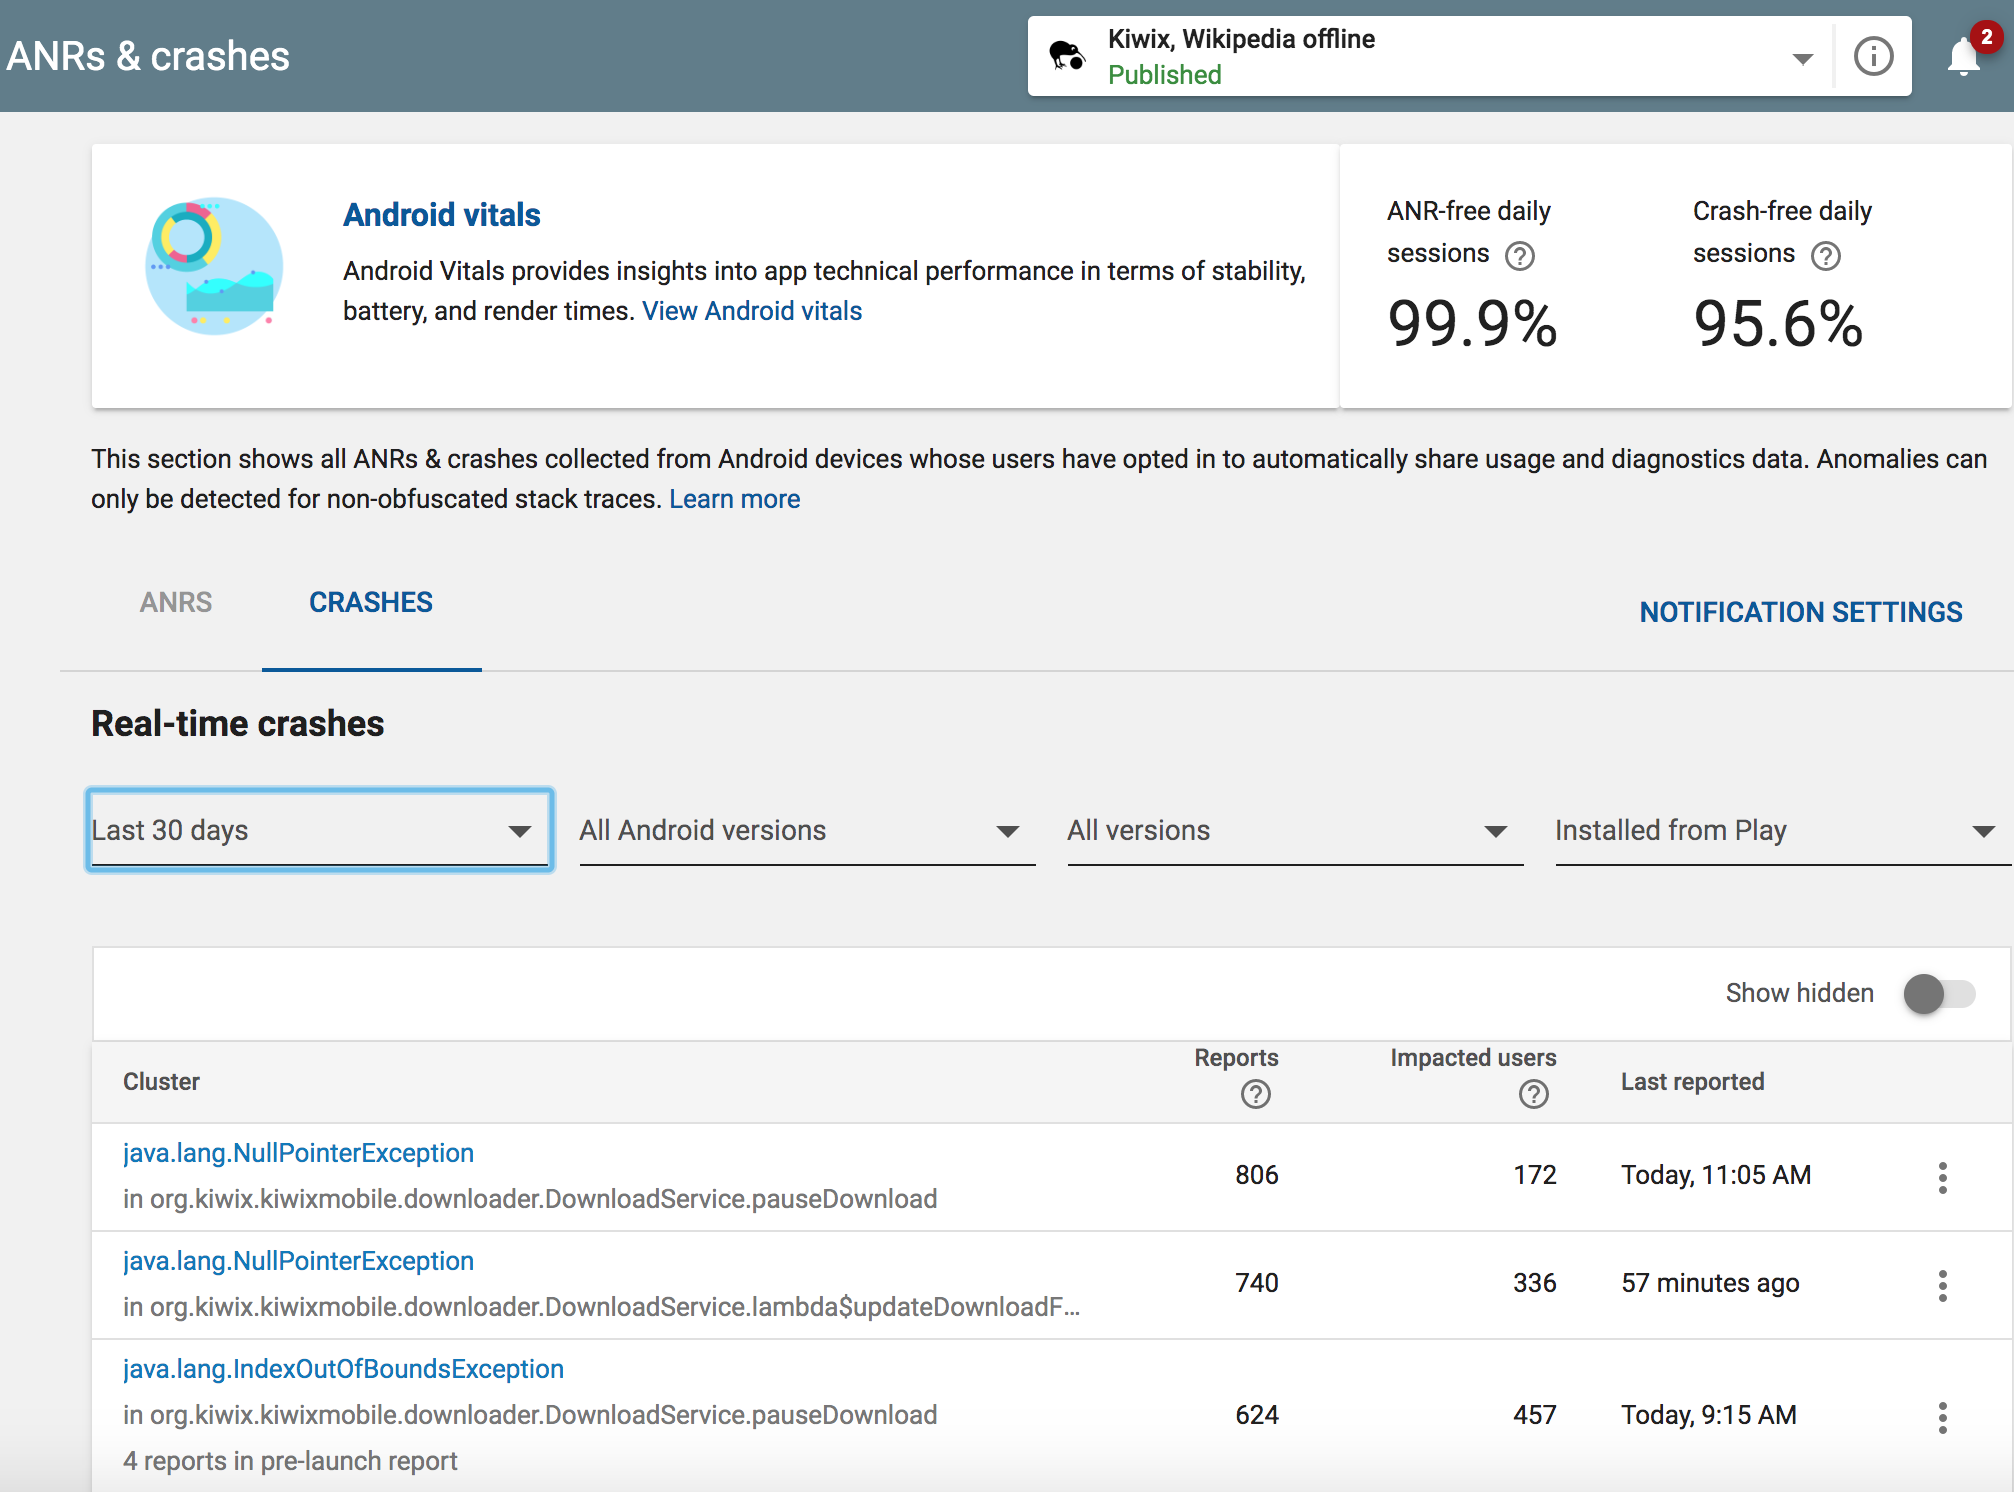
\includegraphics[width=13cm]{images/android-vitals-screenshots/Example-crash-clusters 10-jun-2019.png}
    \caption{Android Vitals: Kiwix Android crash clusters snapshot on \nth{10} June 2019}
    \label{fig:android-vitals-kiwix-android-example-crash-clusters-10-jun-2019}
\end{figure}

In March 2019, we~\footnote{The Android project leads at that time and myself} decided to focus on using analytics to effect improvements in the main Kiwix app and use WikiMed in English as the control. 
\begin{itemize}
    \item There were several reasons for selecting the Kiwix app as the experiment: it contained all the functionality\footnote{baring a tiny amount of code used in the custom apps} and it could process all the contents that the various custom apps contained therefore just about any of the current crashes could potentially be addressed through working on this app. Furthermore as the custom apps were derived from this app fixes in the codebase for the Kiwix app could percolate to the custom apps in future. 
    \item WikiMed in English was the second-most popular app in the family and was highly representative of many of the custom apps in terms of the contents and the likely usage.
\end{itemize}

We chose not to select the Chemistry \& Physics simulations as the contents were highly specific~\footnote{Furthermore, at the time the JavaScript libraries used in the simulations had high demands and would not run as-is on older Android devices. One of the Kiwix developers used a transpilation step to enable the simulations to run on these older devices, nonetheless the simulations were sometimes slow to load and less reliable than we desired. Again, all challenges that were well worth addressing (and the team did so), however they meant we chose not to use this app in the experiment.} 
and if we focused on fixing crash clusters specific to this app they may not effect improvements in the crash rates of many of the other apps in the family. (To be clear, we agreed the specific crashes were still relevant and would be worth addressing, however they weren't the main focus of the work.) 

Three bug clusters were identified through the analysis: the download manager, Android Lifecycle management, and content processing. The development lead was pressed for time and believed the causes of these bug clusters were hard to address. Various approaches were considered including paying for some off-shore developers to sift through the code for clues of the causes; however these were not followed through, partly because of the perceived complexity of a) solving the bugs, b) ensuring they were actually fixed, c) integrating with the Android platform. 
% See email conversation https://mail.google.com/mail/u/0/?q=kiwix+crash+rate+#search/kiwix+crash+rate/QgrcJHrhsvdVtDQRKfRGJrZmpsMLLCfQJcL

\subsubsection{Crash reproduction mini-experiments} 
Two mini-experiments were established during this case study with the aim of evaluating crash reproduction of crashes reported by the mobile analytics. These were: 1) testing interactively on a physical device 2) using CrashScope as the authors of that research claimed it was effective at reproducing crashes.

\textbf{Mini-experiment: device-specific interactive testing} 
Android Vitals sometimes includes the crash rate for specific device models when Google has sufficient data to publish this statistic for that device. One of the devices with a high crash rate was a sm-g532 model. This is a Samsung phone. The model code matches several branded models. As part of the research I decided to procure one of these devices to determine whether crashes could be reproduced when using this device.  

\textbf{Method}: Various sources are available online to map the model code to the branded models. For this case study \url{https://desktop.firmware.mobi/} was used, and one of the matching models was purchased: the Samsung Galaxy Grand Prime Plus Black G532 8GB. 

The then current version of Kiwix was installed on this device~\footnote{Current and historical releases of the Kiwix app are freely available online at \url{http://download.kiwix.org/release/kiwix-android/}.} and the app was used interactively with the aim of triggering one or more of the crashes being reported in Android Vitals. We were not able to explicitly reproduce any of the reported crashes during several sessions of testing over several weeks. 

\textbf{Results}: Given the volume of that testing the results are not definitive and it would be inappropriate to form conclusions from this testing. Percentages over a population of sessions do not necessarily distinguish between a subset of users who have perennial crashes consistently or crashes that occur less frequently over a larger portion of the userbase. There may be other, currently unknown contributory factors that led to the crashes for users on those device models.

\textbf{Mini-experiment: using CrashScope}
The aim of this experiment was to see if CrashScope can trigger some of the crashes automatically that are reported in Android Vitals (part of the Google Play Console). A version of CrashScope is available online~\footnote{at~\url{http://173.255.245.197:8080/CrashScope/index.xhtml}, obtained from the project's homepage~\citep{crashscope_project_homepage}}. In~\citep{moran2016_automatically_drr_android_app_crashes} the authors were able to find distinct crashes with CrashScope compared to other automated testing tools and their automatically bug-reproduction reports were well liked by the students who used them to try to reproduce these crashes (which they frequently managed to do). However, \textit{the crashes it found were not necessarily crashes that occur for end users and there was little indication whether it could find crashes that are occurring for end users.} 

Therefore, it seemed a useful experiment would be to determine whether CrashScope could reproduce actual crashes that affected end users; particularly given the subsequent publication on CrashScope being a practical tool for automated testing of Android applications~\citep{moran2017_crashscope_a_practical_tool_for_automated_testing_of_android_apps}.  Furthermore, as the Kiwix Android codebase is opensource and the apps are popular the experiment could help explore the utility of CrashScope in terms of its use for real-world, popular, Android apps.

\textbf{Method}: An account was created on the public CrashScope site. Two of the Kiwix Android apps were uploaded as APK files: 1) the \href{https://play.google.com/store/apps/details?id=org.kiwix.kiwixcustomphet}{Chemistry and Physics Simulations app} (known as PhET), and 2) the core Kiwix app. The PhET app was downloaded using an online service, APKCombo~\citep{apkcombo_website_about_us}, that facilitates such downloads; and it was used as the PhET app, like all the Kiwix Android custom apps, uses expansion files~\citep{apk_expansion_files} containing the contents. The expansion files are packaged using the Android specific OBB format
%
\footnote{The URL used to download the app was \url{https://apkcombo.com/en-gb/chemistry-physics-simulations/org.kiwix.kiwixcustomphet/download/obb} to download the APK and then the \href{glossary-obb-file-format}{OBB} file for the app. Their website explained how and where to copy the OBB file for the app to access it (they need to be in a particular location for the app to find the contents of the expansion file.}.

\textbf{Results}: 
CrashScope had no facility to upload, include, or use expansion files. I contacted one of the authors of the project, at the time it was not practical for them to add support which meant CrashScope was (and still is not) able to test any apps with expansion files.

The Kiwix app did not appear in their user interface and there were no indications the app had been tested by CrashScope. Similarly I contracted the same author of the project at the time and subsequently. For various reasons, unfortunately, they have been unable to provide a viable environment or any version of CrashScope either in source code or binary formats~\footnote{The authors had intended to make the project available as an opensource project.}.

\textbf{Summary of mini-experiments}
Neither of the mini-experiments were successful at reproducing crashes reported in the field. In the author's experience app developers~\footnote{The practical limitations of being able to reproduce crashes is also corroborated by numerous \textit{ad-hoc} informal discussions with development teams for many apps in industry.} are frequently faced with failures they are not able to reproduce practically. This indicates app development teams may need other practical mechanisms to determine whether failures have been ameliorated or even fixed. Concepts such as relative correctness e.g. in~\citep{ghardallou2016debugging_without_testing} show promise in terms of comparing the failures reported in subsequent releases of an app, the absence of a particular failure \textit{might} indicate the failure has at least been partly addressed provided the developers have made attempts to address at least one possible cause of the failure. In some instances, failures have remained submerged for several releases - for instance with the Kiwix Android app, in September 2019 there were 55 crashes reported for a \texttt{WebViewFactory MissingWebViewPackageException}; see Figure~\ref{fig:55-crashes-missing-webview-package-exception}. This crash disappeared for several releases before reappearing. The disappearance might have been for various reasons, one possible one was simply the particular user who was adversely affected stopped using the app. 

\begin{figure}
    \centering
    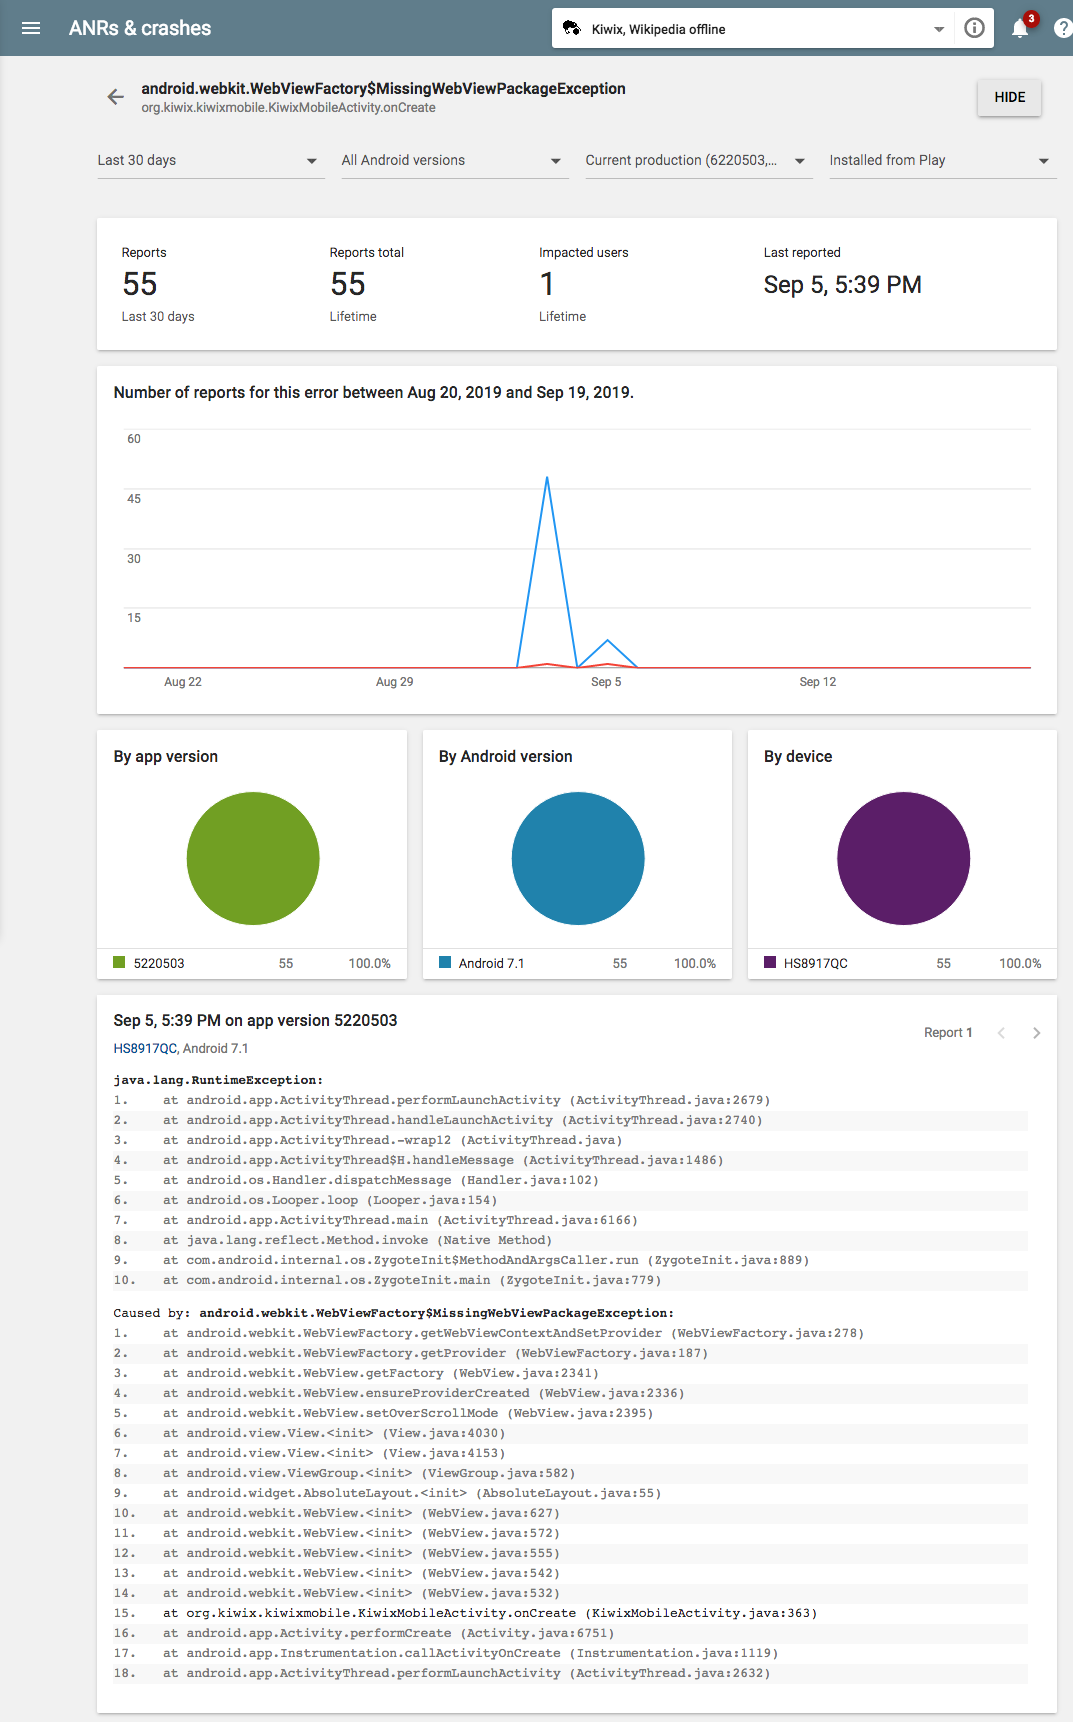
\includegraphics[width=13.5cm]{images/android-vitals-screenshots/55-crashes-WebViewFactory-MissingWebViewPackageException_2019-09-19-kiwix_trimmed.png}
    \caption{Kiwix Android 55 crashes for one user}
    \label{fig:55-crashes-WebViewFactory-MissingWebViewPackageException}
\end{figure}

\FloatBarrier

\subsection{Results/Outcomes}
\textit{(Describe the outcomes resulting from the intervention). Not the speculative analysis, here it’s the concrete analysis of what was done.}

\begin{figure}
    \centering
    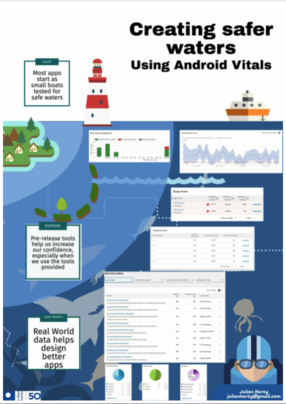
\includegraphics{images/mobilesoft/resized-mobilesoft2019-poster.png}
    \caption{MobileSOFT 2019 Poster}
    \label{fig:mobilesoft2019-poster}
\end{figure}

Remember to write up and include the figures and screenshots from both MobileSOFT 2019 (Figure\ref{fig:mobilesoft2019-poster}) and MobileSOFT 2020 (Figure~\ref{fig:mobilesoft2020-poster}.

Some useful snapshots of the improvements are in my JioConf November 2020 keynote of the crash rate for Kiwix. TODO.

%\akb{The unsuccessful mini experiments make it hard to pick out which of the analytics related actions contributed to the first outcome reported below}

This case study led to several distinct forms of outcomes. The first was the dramatic improvement in the crash rate of the experiment app - Kiwix. The second was the development and adoption of opensource software - Vitals Scraper - which facilitated the collection and retention of otherwise ephemeral analytics information. And the third was the collaboration with the engineering team for Google Play Console as we discovered and reported various flaws in Google Play Console and Android Vitals. 

The mini-case studies did not provide direct outcomes (as neither provided the intended results). Instead they provided a couple of indicators that inform ongoing engineering practices and research. The first indicator, is that some failures may be impractical to reproduce within the time and other resources available at the time to the development team. Analytics tools such that measure [un-] reliability may help those teams measure the effects of their changes once the release is being used. The second indicator is that even promising research tools may also be impractical to apply beyond the immediate ecosystem that created that tool or after that research was published. The group that created CrashScope also provided a running instance of it at the time, however the service has not functioned on demand and the underlying software isn't available for others to use. Opensourcing the code of such tools provides an incomplete approach to enabling others to use and reuse the work. The code needs to include adequate support and ideally be maintained on an ongoing basis, something that seldom occurs for a multitude of reasons.

%%%% Table generated originally by Spread-LaTeX
%\begin{adjustwidth}{-1 cm}{-1 cm}
\begin{threeparttable}[!htp]\centering
\caption{Reductions in Crash Rates}\label{tab:kiwix-evaluation-reductions-in-crash-rates}
\scriptsize
\begin{tabularx}\textwidth{llrr} % SHOULD-DO I'd like to reduce the width slightly.
\toprule
%& & & & \\
&\multicolumn{3}{c}{30-day crash rates reported in Android Vitals~\tnote{0}} \\
\midrule
\multirow{2}{*}{.} &\multicolumn{2}{c}{Kiwix Apps} \\
Stage &Release&\cellcolor[HTML]{efefef}Experiment &Control  \\

&\cellcolor[HTML]{efefef}&\cellcolor[HTML]{efefef}Kiwix & WikiMed English \\

1 &0 
  &\cellcolor[HTML]{efefef}5.07\% &1.13\% \\
2 &1 &\cellcolor[HTML]{efefef}3.12\%~\tnote{1} &\multirow{2}{*}{\cellcolor[HTML]{A8A8A8}}... \\
3 &2~\tnote{2} &\cellcolor[HTML]{efefef}1.59\%~\tnote{3} & \cellcolor[HTML]{A8A8A8}... \\
  &3 &\cellcolor[HTML]{efefef}0.53\%~\tnote{4} &1.09\%~\tnote{5} \\
4 &4 &\cellcolor[HTML]{efefef}0.72\%~\tnote{6} &0.60\%~\tnote{7} \\
  &4~\tnote{8} 
&\cellcolor[HTML]{efefef}0.55\% &0.41\% \\
  &5 &\cellcolor[HTML]{efefef}0.40\%~\tnote{9} &0.26\%~\tnote{10} \\
\bottomrule
\end{tabularx}
\begin{tablenotes}
  \item[0] Except when otherwise noted.
  \item[1] Kiwix Release 2.5 with the previous custom download facility replaced by a Google Android downloader.
  \item[2] The code is under 25 lines including 10 lines of comments~\url{https://github.com/kiwix/kiwix-android/pull/1388}.
  \item[3] Aggregate crash rate over 7 days for versions 2.4, 2.5.1, 2.5.2, 2.5.3 (to Aug \nth{26} 2019).
  \item[4] Previous 30 days crash rate, before release 3.1.2 pushed the crash rate up (same graph as TODO).
  \item[5] \emph{Unchanged release from the first control.}
  \item[6] Includes 3.1.2 which had an average (mean) crash rate of roughly 1.7\% (roughly \nth{31} Dec 2019).
  \item[7] A mixed set of crash rates, averaged by Android Vitals. For the first updated release of Wikimed (the 2019-12 release).
  \item[8] As usage increased of the more reliable releases the averages declined.
  \item[9] The crash rates for releases 3.2.1 are 0.23\% and 3.3.1 are 0.31\%
  \item[10] Release 2020-03 actually has a crash rate of around 0.05\% the numbers are higher as there are still significant volumes of usage on the previous 2 releases.

\end{tablenotes}
\end{threeparttable}
%\end{adjustwidth}
\vspace{5mm}
%%%% Isabel recommends creating a timeline instead - sounds good SHOULD-DO

Table~\ref{tab:kiwix-evaluation-reductions-in-crash-rates} provides a comparison of the crash rates for the experiment and the control apps over four stages of this case study. There were three phases that interleave with these four stages.

The stages are:
\begin{enumerate}
    \itemsep0em
    \item The baseline,
    \item Simplifying the most buggy code (which was the downloader),
    \item Applying the concepts in the research to the experiment,
    \item The new normal.
\end{enumerate}
% Great ideas to reduce space in list items in https://tex.stackexchange.com/questions/6081/reduce-space-between-enumerated-items
% COULD-DO I've only applied the basic suggestion for this single list so far, might be worth thesis wide changes as the thesis matures.

The active part of the experiment started in stage 3 of this case study, although the initial research into the feasibility started several months earlier during the baseline stage.

\subsection{Stage 1: the baseline}
Before the experiment started there was little focus on finding and fixing causes of crashes. The development team did fix some sporadically, however they seldom used the reports from Android Vitals to identify crashes or address them.

The core app included an integrated download facility to download content to a user's local device. Files sizes ranged from a few MB to over 60GB and could take several days to download, especially in areas where connectivity wasn't ideal.  This integrated download facility provided users with several useful features, for example, they could pause and restart downloads. It also had an integrated recovery mechanism to restart and continue partial downloads after a failure, and it provided users with a progress indicator. However, this custom download facility had numerous bugs and was the largest source of crashes in real world use.

The custom apps were pre-packaged with content (which Google Play Services downloaded at the same time as downloading the app's binary). They did not need, and did not include the custom downloader. This meant their crash rates were significantly better (lower) than the core app managed.

\subsection{Stage 2: simplifying the most buggy code}
The first release, release 1 in the table, predated the hackathon (which was the start of the experiment). In this release the lead developer decided to replace a large body of custom code with generic downloader code rather than focus on fixing individual sections of code~\footnote{The combined commit with this change is~\href{https://github.com/kiwix/kiwix-android/commit/fcac33cf2daed5cea98387743c5c5dc52d59e09a}{commit fcac33cf2daed5cea98387743c5c5dc52d59e09a}}. The custom code was considered too problematic to fix. However, there was a trade-off by increasing the reliability there was a reduction in usability and also an impact on what happened when downloads stopped or otherwise failed before completion. The crash rate reduced to under 2\% once most users had the release with the new downloader installed.

\subsection{Stage 3: applying the research concepts of the experiment app}
I convinced the the leaders of the Kiwix project that we might be able to reduce the crash rate significantly by applying the concepts described in chapter 5. They had slowly become increasingly aware of the excessively high crash rate and the potential impact on both users and the app store's ranking of the apps based on the high crash rates. 

We agreed we would start by focusing on several of the most frequently occurring crashes as reported in Android Vitals. The opportunity to do so was at a week-long hackathon in Stockholm in August 2019~\footnote{A summary of the overall hackathon is available online \url{https://wiki.kiwix.org/wiki/Hackathon_Wikimania_2019}}. I led the discussions and analysis with several of the volunteer developers at the hackathon.

Following this discussion and analysis about the crashes being reported in Android Vitals for version \texttt{2.5.0} of the core application, the developers fixed several of the causes of the most frequent crashes with a surprisingly small amount of code of under 25 lines (including 10 lines of text added to the release log)\footnote{\url{https://github.com/kiwix/kiwix-android/pull/1388}}. Of interest, at least one of the fixes had actually been made and committed to a pending major release of the app but wasn't applied to the current production release~\emph{until the effects of the crash was made visible using analytics}. Details of the crash report and fix are available online~\url{https://github.com/kiwix/kiwix-android/issues/1261}~\footnote{The release was rolled out in Google Play to end users in stages from \nth{19} to \nth{23} August 2019 in stages, through an overabundance of caution given the small footprint and nature of the changes.}. The crash rate stabilised around 1.1\% once the majority of userbase had release 2.5.3 installed; it would have been lower were it not for the \texttt{UnsatisfiedLinkError} exceptions, discussed next.

Several new crash clusters emerged for \texttt{UnsatisfiedLinkError} exceptions. These were not directly related to the crash fixes in the \texttt{2.5.x} releases, instead they were related to the project choosing to apply advice from Google to use App Bundles~\citep{android_app_bundle}~\footnote{In practice, app releases often include a mix of bug fixes together with other changes so it is sometimes impractical to measure the effects of bug fixes in isolation. Similar challenges and behaviours exist in code commits,~\citep{partachi2020_flexme_untangling_commits} discusses that topic well. Nonetheless approaches used to detangle commits are unlikely to work as-is for releases as releases need to satisfy other constraints. Release planning and release management are discussed in~\href{chapter-related-work}{\nameref{chapter-related-work}}}.
%
With App Bundles Google Play took responsibility for delivering the correct app binaries to suit the end-user's device's hardware architecture~\emph{e.g.} ARM 32-bit, ARM-64 bit, Intel 64-bit, and so on. However, sometimes the users seemed to receive one or more binaries that didn't run on their device which led to this crash. What wasn't well published is enabling App Bundles is similar to Caesar crossing the Rubicon~\footnote{\url{https://grammarist.com/idiom/cross-the-rubicon/}} - there's no turning back. Therefore, rather than having the option to revert to `fat binaries' the project had to find an approach that worked in the context of App Bundles. As the Kiwix Android apps include a native library, written in C++, the solution needed to work for native code in addition to managed code.

There's quite a detailed issue report available on GitHub.com,~\href{https://github.com/kiwix/kiwix-android/issues/1259}{Issue 1259 - Crash Report: \texttt{UnsatisfiedLinkError} reported in Android Vitals for 2.5.x users}. The cause required in-depth investigation, changes to the build process, and changes to the application code in order to reduce the likelihood of the incorrect binaries being deployed to the end user devices.

Various developers continued to make corrective changes to the codebase which made ongoing incremental improvements to the app released to the \texttt{2.5.x} releases.

\subsection{Stage 4: the new normal}
The improvements in the reliability of the core app were sufficiently compelling \emph{and} the reliability of the custom apps sufficiently poor that the development team chose to refresh the majority of the custom apps, including the one used as the control (WikiMed English). Note: Various details of the crash rate at the time and the plan to migrate the custom apps are included in~\url{https://github.com/kiwix/kiwix-android/issues/1426}. 

All the apps share a common codebase, they are created using a common set of build scripts, they differ in their data contents, various `resources'~\footnote{\emph{``Resources are the additional files and static content that your code uses, such as bitmaps, layout definitions, user interface strings, animation instructions, and more."}~\url{https://developer.android.com/guide/topics/resources/providing-resources}}, and the custom apps exclude file management and download features as the contents are pre-packaged as part of the build process instead.

Several releases later, each with various changes and improvements aimed at fixing causes of crashes the crash rate was materially lower than when we started, at the time of writing the overall crash rate for the last 7 days is 0.54\% which is inflated because the rash rate for the previous release (\texttt{3.1.2}) spiked at 1.38\%, compared to 0.18\% for release (\texttt{3.0.5} -  the last production release) and 0.25\% for the recently released fix (\texttt{3.1.3}).



\subsubsection{Improvements in the crash rates}
Improvements in the crash rate came in three phases:
\begin{enumerate}
    \itemsep0em
    \item Replacing the custom downloader with core Android functionality in version 2.5 of the Kiwix app.
    \item Targeted crash fixes found and addressed during a hackathon in Stockholm, Sweden.
    \item Ongoing crash fixes, combined with migration of code from Java to Kotlin.
\end{enumerate}

\textbf{Phase 1}: As reported here and in \cite{harty_google_play_console_insightful_development_using_android_vitals_and_pre_launch_reports} and \cite{harty_better_android_apps_using_android_vitals} the Kiwix Android app had a very high overall crash rate caused by several significant flaws in the app. The project team released version 2.5 of the main Kiwix app in July 2019. As figure \ref{fig:kiwix_crash_rate_drops_v2_5} shows, the crash rate decreased significantly as version 2.5 rolled out to the majority of the userbase. %In the last 30 days the crash rate was 1.87\% down from 5.07\% in February 2019.

One of the major changes in version 2.5 was the replacement of the in-house download utility with the default Android Download Manager\cite{kiwix_release_2_5_0}. The in-house, custom, version was a major source of crashes, and the replacement obviated a class of crashes, however it did so at a price in terms of functionality and usability. The in-house download utility allowed users to pause and resume downloads, and it would complete failed partial downloads. Users also received updates on the progress of the downloads, important when they often took many minutes or even hours or days in some cases (such as for multi-GB downloads over poor, slow, unreliable connections on low-end devices).

\begin{figure}[htbp!]
    \centering
    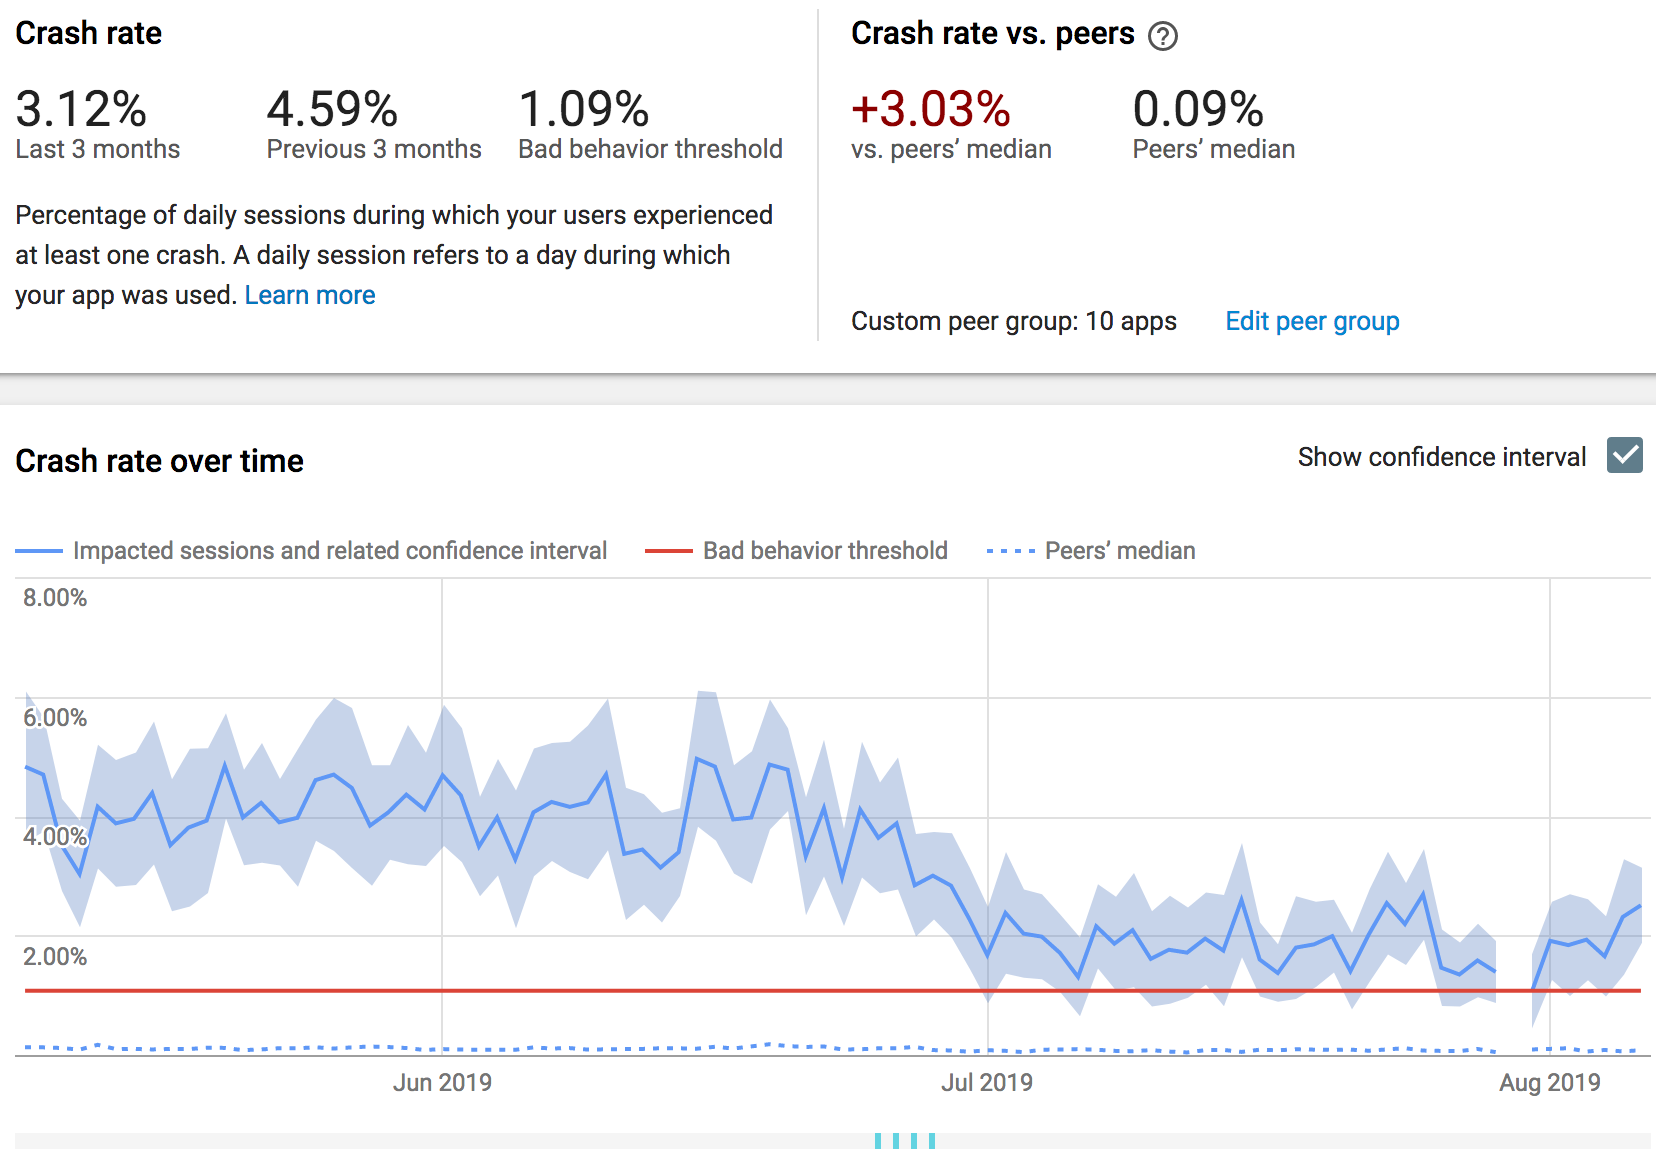
\includegraphics[width=\textwidth]{images/android-vitals-screenshots/kiwix-crash-rate-drops-with-v2_5.png}
    \caption{Kiwix Crash Rate Drops with V2.5 Release}
    \label{fig:kiwix_crash_rate_drops_v2_5}
\end{figure}

\textbf{Phase 2}: Following initial discussions about the crashes being reported in Android Vitals for version 2.5.0 of the Kiwix application, a group of the developers for the Kiwix projects collaborated on a week-long hackathon in Stockholm in August 2019. One of the areas the developers worked on was to focus on identifying and addressing some of the biggest contributors to the high crash rate. 
%

%%%%% Consider whether to convert the following two visual figures to code listings so they can be included in the Code Listings in the table of contents. 
\begin{figure}
    \centering
    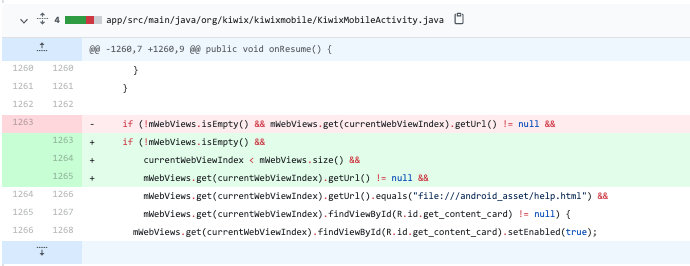
\includegraphics[width=14cm]{images/github/kiwix-pr1388-extract-1.png}
    \caption{First material change in PR-1388 for Kiwix Android}
    \label{fig:kiwix_pr1388_extract_1}
\end{figure}


\begin{figure}
    \centering
    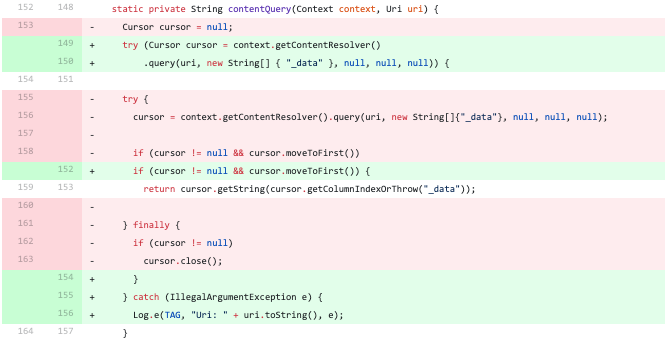
\includegraphics[width=14cm]{images/github/kiwix-pr1388-extract-2.png}
    \caption{Second material change in PR-1388 for Kiwix Android}
    \label{fig:kiwix_pr1388_extract_2}
\end{figure}


The developers ended up fixing some of the causes of the most frequent crashes with a surprisingly small amount of code of under 25 lines (including 10 lines of text added to the release log)\footnote{\url{https://github.com/kiwix/kiwix-android/pull/1388}}. Figures~\ref{fig:kiwix_pr1388_extract_1} and~\ref{fig:kiwix_pr1388_extract_2} illustrate the material changes that were made to address two of the crashes. The first adds another null check: \small{\texttt{currentWebViewIndex < mWebViews.size() \&\&}}. 
The second catches an \texttt{IllegalArgumentException} if one occurs. 

According to Android Vitals, the crash rate was more than halved once release 2.5.3 had rolled out to the majority of the userbase, for example for the 30-day period of \nth{19} Aug 2019 to \nth{16} Sep 2019 the overall crash rate was 1.47\% for the Kiwix app. Figure~\ref{fig:kiwix_android_vitals_with_gaps_2019_09_20} is the source of this data. Several aspects of this figure will be discussed in more detail in the \href{section-flaws-in-the-analytics}{\nameref{section-flaws-in-the-analytics}} topic. For now, the main point to highlight in this figure is the difference between the crash rates for two different builds of the 2.5.3 release, 0.96\% for 6220503 versus 2.22\% for 5220503. These builds were for different hardware architectures of Android where crashes related to Android App Bundles occurred more often for the 5220503 release. Further analysis of these crashes are in the~\href{kiwix-android-app-bundling-crashes}{\nameref{kiwix-android-app-bundling-crashes}} topic.

\begin{figure}
    \centering
    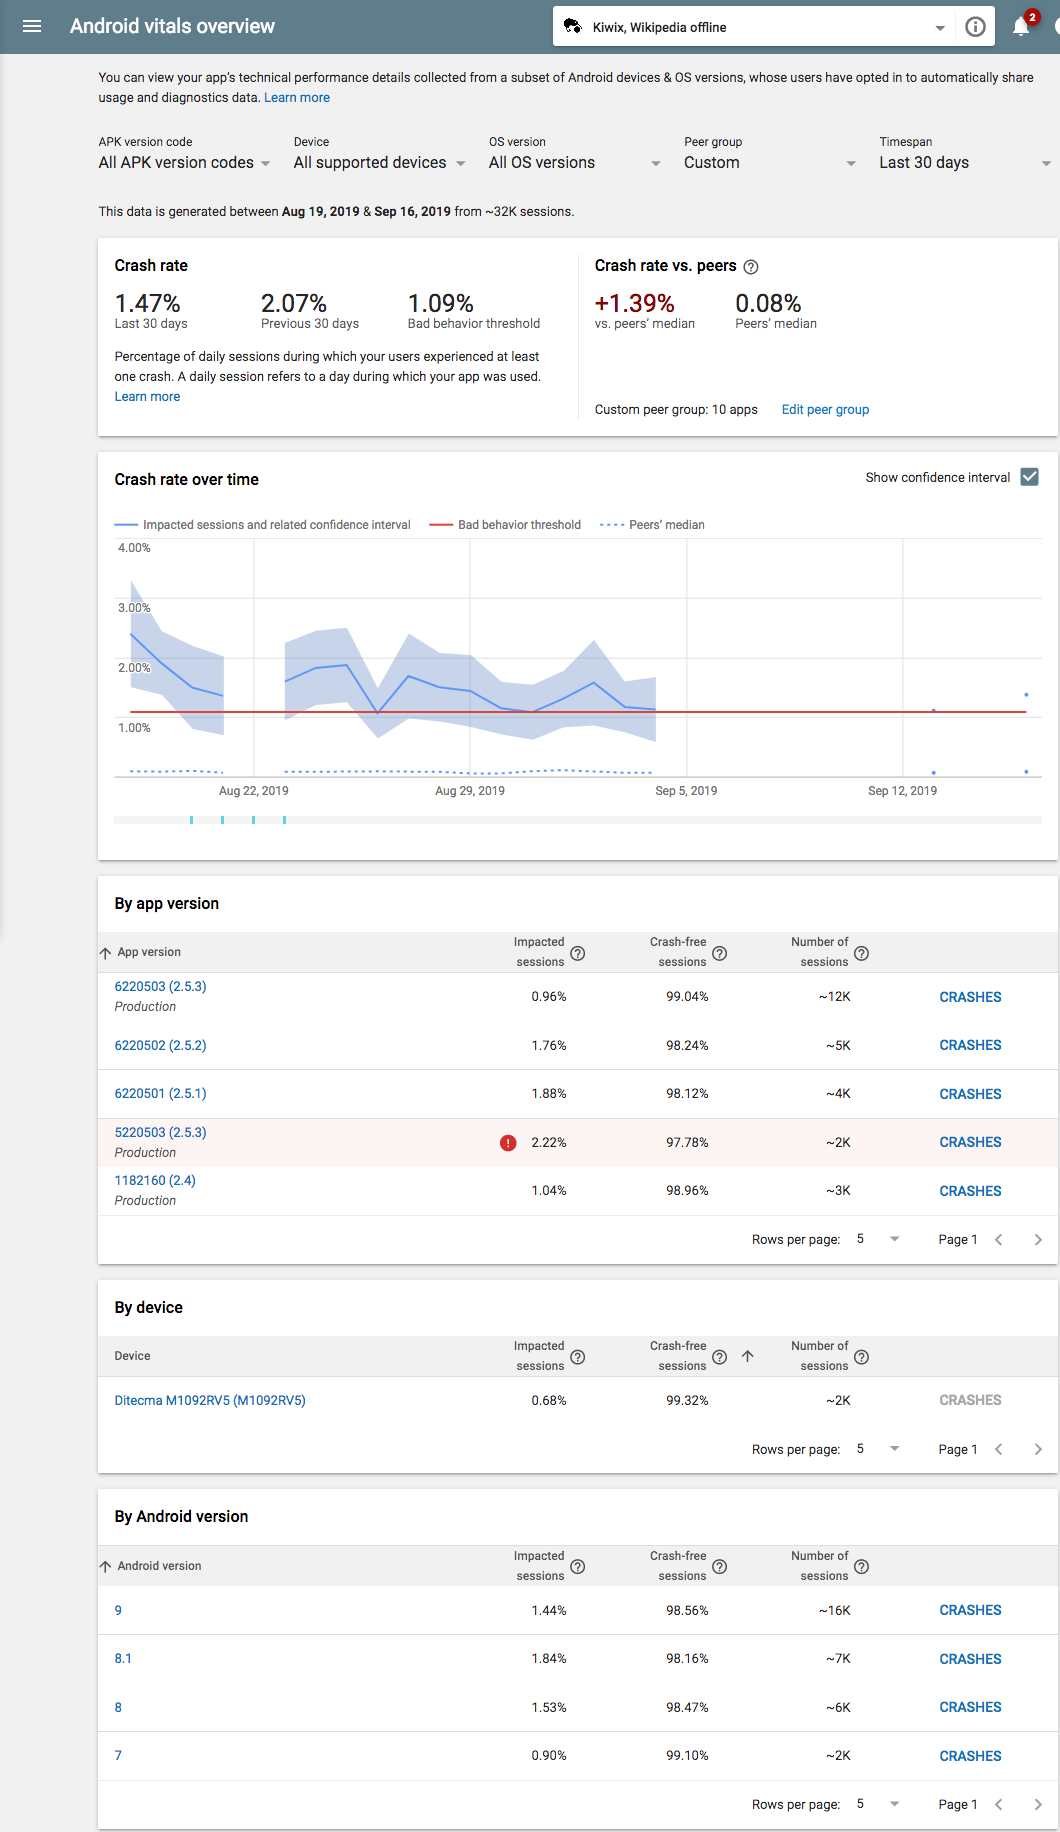
\includegraphics[width=12.5cm]{images/android-vitals-screenshots/Screeenshot_2019_09_20_Android_Vitals_Overview_Kiwix_Google_Play_Console.png}
    \caption{Android Vitals overview for Kiwix, 30 day view on \nth{20} Sep 2019}
    \label{fig:kiwix_android_vitals_with_gaps_2019_09_20}
\end{figure}


Various developers continued to make corrective changes to the codebase which made ongoing incremental improvements to the app released to the \texttt{2.5.x} releases. 



\textbf{Phase 3}: Several developers for the Kiwix project, the lead developer in particular, have been actively reviewing crashes reported by Android Vitals, filing issues, and addressing the causes of the crashes in order to reduce the crash rate and improve the app's stability. For the Kiwix project crashes are tracked as issues on GitHub, on~\nth{11} June 2021 there are 182 closed and 8 open issues that mention `crash': 182 closed, 8 open % Was 133 closed, 6 open.
\footnote{\url{https://github.com/kiwix/kiwix-android/issues?q=is\%3Aissue+crash}}
%COULD-DO analyse each issue to identify the source of the crash.

Several releases later, each with various changes and improvements aimed at fixing causes of crashes the crash rate was materially lower than when we started, in early 2020 the overall crash rate for the last 7 days was 0.54\% which is inflated because the rash rate for the previous release (3.1.2) spiked at 1.38\%, compared to 0.18\% for release (3.0.5 -  the last production release) and 0.25\% for the recently released fix (3.1.3).


\textbf{A Quick discussion on perspectives and views}. 
One of the key challenges when trying to interpret Android Vitals analytics is to determine comparisons and to establish reference points. For instance, are the recent crashes related to the embedded WebView component related to changes in the app, in the Android platform, to a particular device manufacturer? 

For instance, the most frequent crash in the 60 days to \nth{11} Jun 2021 has only occurred on Huawei devices for the most recent release of the Kiwix app (3.4.4). The nub of the crash is in Listing~\ref{listing:kiwix-app-crash-3-4-4}

\begin{lstlisting}[language=java, caption=Extract of stack trace for the most frequent crash in release 3.4.4 of Kiwix, label=listing:kiwix-app-crash-3-4-4]
java.lang.IllegalStateException
org.kiwix.kiwixmobile.core.main.CoreReaderFragment.webViewFailedLoading
\end{lstlisting}

that affected 16 users a total of 96 times in these 60 days. % https://play.google.com/console/developers/9116215767541857492/app/4975184706939091905/vitals/crashes?errorType=CRASH&versionCode=6230404%2C5230404%2C4230404%2C3230404&days=60&installedFrom=PLAY_STORE
Could this be related to The US government's ban on Huawei including the prevention of Google software from being installed on new Huawei models?~\footnote{\url{https://www.cnet.com/news/huawei-ban-timeline-chinese-company-android-rival-coming-phones-tablets/}~\citep{androidauthority2021_the_huawei_ban}, \url{https://www.androidauthority.com/huawei-google-android-ban-988382/}} and/or the Android WebView component being disabled, or yet another as yet unknown cause? (For instance perhaps it's a similar crash to the one reported on some models of Samsung S9 and S9+ phones~\citep{ebling2018_so_s9_specific_webview_device_crash_report}? Understanding the reasons may help the developer decide on a suitable method to address the runtime failure in the app and/or provide a better user-experience.

% Some notes are in a the draft materials document in \href{section-experiments-with-webviews}{\nameref{section-experiments-with-webviews}}.



\subsubsection{Vitals Scraper}
~\href{section-vitals-scraper}{\emph{Vitals Scraper}} was developed to facilitate the collection, preservation, and sharing of reports and data presented in Google Play Console and Android Vitals. Details of the software's design and implementation are discussed in the~\href{chapter-code-needed}{\nameref{chapter-code-needed}} chapter.

\begin{figure}
    \centering
    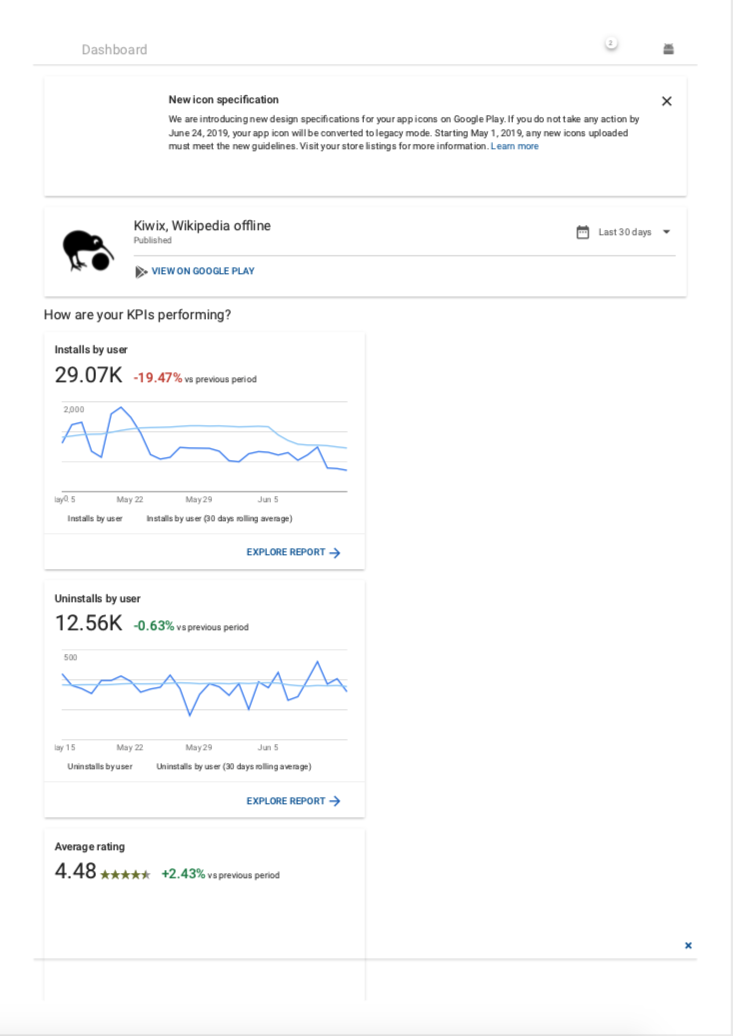
\includegraphics[width=7cm]{images/google-play-console/Dashboard - Kiwix-Google-Play-Console-(2019-Jun-14)-p1.png}
    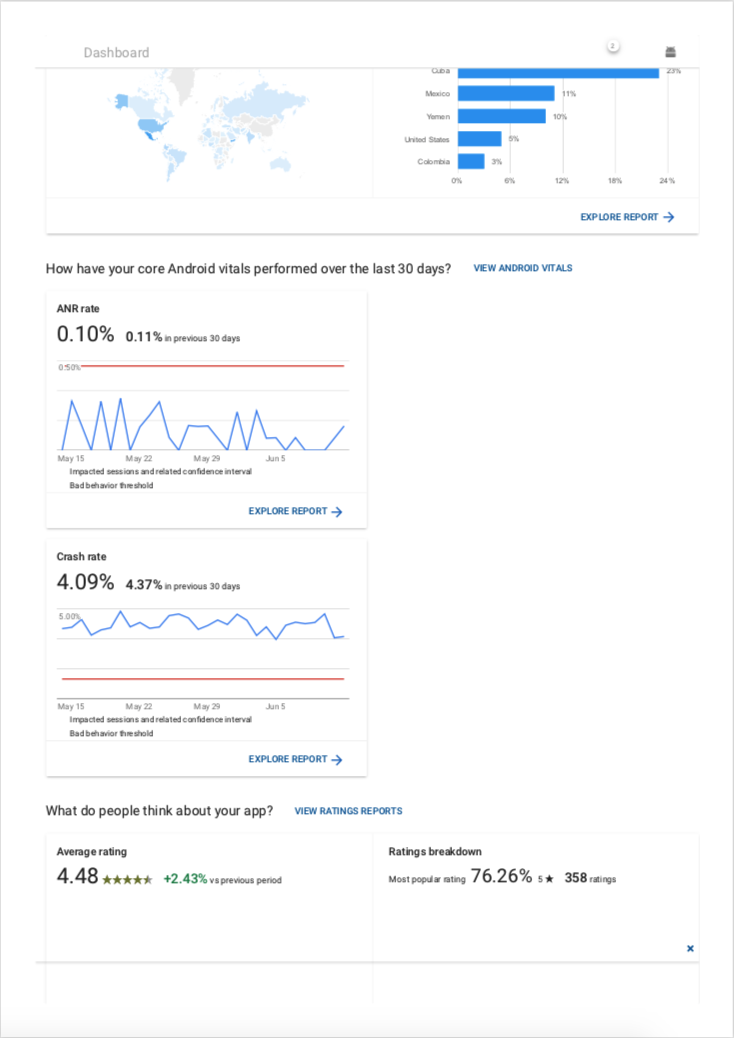
\includegraphics[width=7cm]{images/google-play-console/Dashboard - Kiwix-Google-Play-Console-(2019-Jun-14)-p3.png}
    \newline
    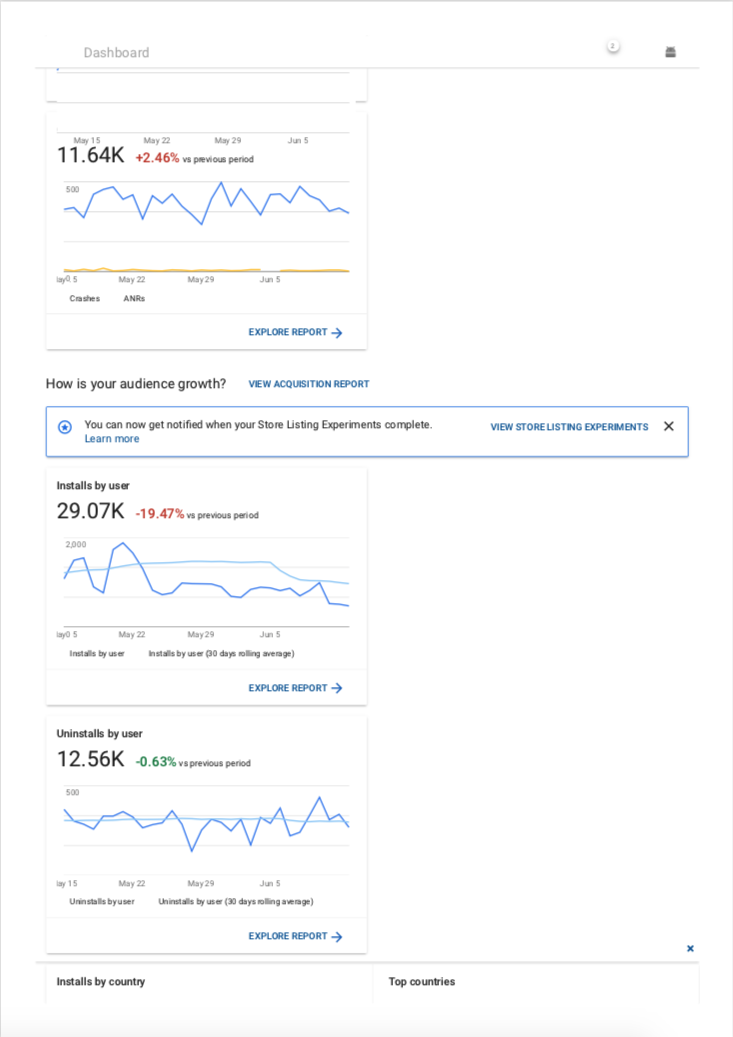
\includegraphics[width=7cm]{images/google-play-console/Dashboard - Kiwix-Google-Play-Console-(2019-Jun-14)-p2.png}
    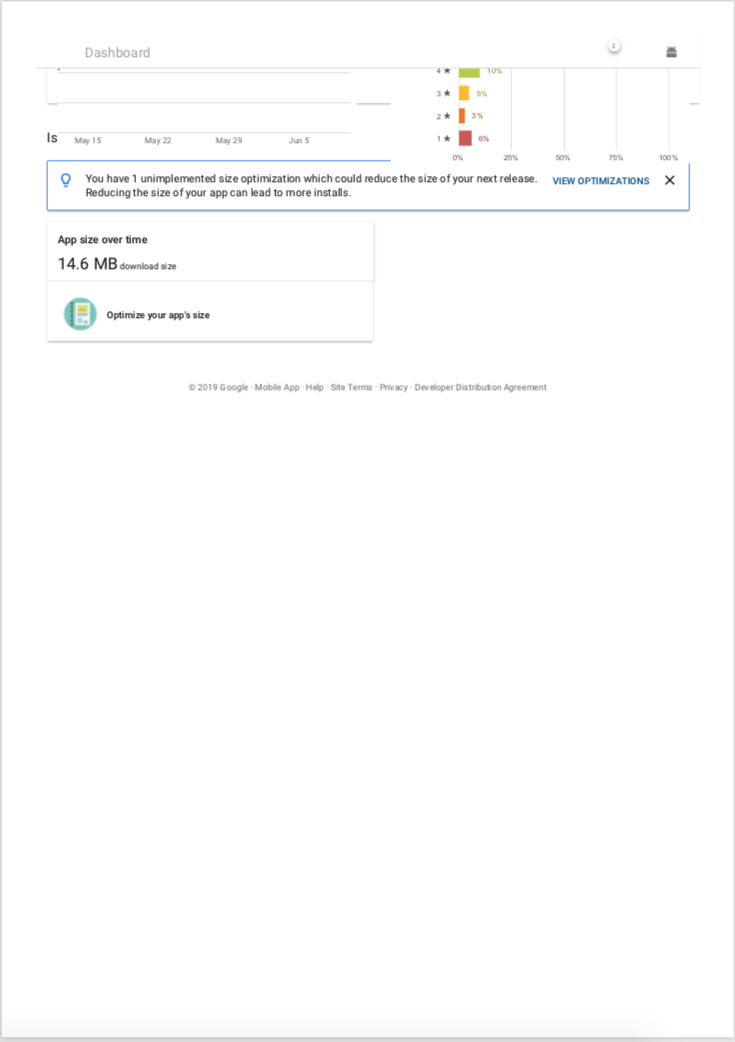
\includegraphics[width=7cm]{images/google-play-console/Dashboard - Kiwix-Google-Play-Console-(2019-Jun-14)-p4.png}
    \caption{Print web page of Dashboard in Google Play Console}
    \label{fig:screenshot-dashboard-gpc-kiwix}
\end{figure}

To help illustrate why tools such as Vitals Scraper was developed, Figure~\ref{fig:screenshot-dashboard-gpc-kiwix}, shows the results of printing the dashboard for the Kiwix app in Google Play Console on \nth{14} June 2019, in order to record the analytics reports for the app. Content is poorly formatted and split across pages, and web page pop-ups sometimes overlaid and obscured the contents of the report. (Some of the flaws illustrated in the contents of the report will be discussed shortly).

Vitals Scraper was able to extract data from various on-screen reports that wasn't otherwise available. It also generated cleaner reports saved as images. Vitals Scraper was jointly developed with Joseph Reeve as an opensource project and tested independently by a lead developer of one of the commercial app projects mentioned later in this thesis as part of evaluating the applicability and generality of the software. It could be scripted and run unattended to facilitate data collection at scale and as an ongoing basis.

In terms of this research, Vitals Scraper was used to collect analytics reports for multiple projects and development teams including the Kiwix apps. 


\subsubsection{Flaws in the analytics}~\label{section-flaws-in-the-analytics}
Various flaws and/or limitations were discovered in the analytics through using them. Their discovery led eventually to collaborating with the relevant engineering team at Google who were responsible for the analytics and for Google Play Console, which is discussed in the next topic.

You may already have noticed that the previous two figures both contain visible flaws. Figure~\ref{fig:kiwix_crash_rate_drops_v2_5} has a gap in the graph, and figure~\ref{fig:screenshot-dashboard-gpc-kiwix} already illustrates at least one flaw, where two reports (the installs by user and uninstalls by user) were repeated in the dashboard for the Kiwix application (on the first and second pages of the print out). 

Fourteen of the flaws were published in a poster that supported my short paper at MOBILESoft 2020~\citep{harty_improving_app_quality_despite_flawed_mobile_analytics}. The flaws discovered in Google Play Console and Android Vitals are also itemised in Table~\ref{tab:issues-in-google-play-console-reports} in the discussion chapter which combines flaws from several case studies.

A key consideration is to determine if they were local in scope or more general. They were cross-checked in several dimensions:
\begin{itemize}
    \item Across apps on the same Google Play Console account.
    \item Across multiple Google Play Console accounts.
    \item For other logins.
    \item With the engineering team who created and provided the analytics service. 
\end{itemize}

All of these checks eventually use the same source of analytics data - that gathered by Google Play Services running on end-user Android devices~\footnote{More precisely, by design, the data is collected from Android devices where the device manufacturers have satisfied Google's requirements where those devices have various Google software pre-installed. There ~\emph{may} be additional sources of the data e.g. where Google Apps have been installed subsequently using GApps~\citep{opengapps} or similar services including~\citep{nikgapps}.}.
%
Subsequent case studies extend the comparisons to additional sources of analytics for similar analytics events, particularly crashes.

As some flaws are data dependent sometimes they cannot be checked for every app and every login for every period. On this basis there may be other flaws that I did not experience.

When several of the flaws emerged they were reported to Google through two channels. The first is available to Android developers when they are using Google Play Console, through a feedback menu option in the Google Play Console user interface. The second was through directly contacting a public member of the product team for Google Play Console and Android Vitals, at that time Fergus Hurley. 

\begin{comment}
The bugs include inconsistencies in the crash rate, reported variously as 6.75\%, 5.48\%, and 5.07\% for the main Kiwix app. The values are found in various sections of the data, however, it's not clear why each is favored in particular areas of the Reports.

\nth{14} March 2019
FYI I've also found the counts of Crashes (11.99K) https://play.google.com/apps/publish/?account=9116215767541857492#AppDashboardPlace:p=org.kiwix.kiwixmobile&appid=4975184706939091905  is higher than either the last 30 days of crashes and even the combination of crashes and ANRs (assuming my copy+paste and manual editing didn't lose any data). https://play.google.com/apps/publish/?account=9116215767541857492#StatisticsPlace:p=org.kiwix.kiwixmobile&appid=4975184706939091905&statms=DAILY_ANDROID_METRICS_CRASHES&statms=DAILY_ANDROID_METRICS_ANRS&statg=DAILY&ts=THIRTY_DAYS I've attached the calculations in an Excel spreadsheet so you can check these if you wish.

I've made quite a few changes, partly after a good discussion today with Fergus Hurley at Google who challenged lots of details in the flaws section and wanted as much feedback and suggestions as possible on ways I'd like the tools improved.
\end{comment}

\begin{comment}
Issues reported using Google Play Developer Support on \nth{19} June 2018, Google replied on \nth{19} July 2018, one month later (many times longer than their published response time of a few days at the time).

Please see a copy of your initial inquiry:

"The pre-launch reports indicate the tests aren't actually running these 
days. Instead it states the app is incompatible with all 14 devices with 
the following error message: "Devices incompatible with APK" 

And I had asked for these two items in response:
Which APK version code you wish to view the pre-launch report for?
Screenshot of the page you're viewing(these are really helpful!)

\nth{24} July 2018: 
 I'm still seeing some test runs in the pre-launch report that claim some devices aren't compatible, and also many more test runs that don't seem to run any tests at all. 

It's not obvious why sometimes the number of devices varies - do you have any idea why? e.g. sometimes the tests seem to be scheduled on 9 devices, other times 7, and often 0

I've attached a couple of screenshots.
And here's a URL for the test run with 7 devices
https://play.google.com/apps/publish/?account=9116215767541857492#PreLaunchReportPlace:p=org.kiwix.kiwixmobile&plrtab=CRASH&plrvc=1181980
and here with 9 
https://play.google.com/apps/publish/?account=9116215767541857492#PreLaunchReportPlace:p=org.kiwix.kiwixmobile&plrtab=SCREENSHOTS&plrvc=181980

Also, in case you're interested, the Pixel 2 device sometimes reports an extremely long start up e.g. 16K (presumably milliseconds) as shown in one of the attached screenshots however, watching the video it's clear the tests are interacting with the app and the app is responding within a couple of seconds. This quirk seems to happen mainly on the Pixel 2 - perhaps there's a bug in how it (the device model) reports activity? Any suggestions?

And sorry I realise I didn't provide an example of where the pre-launch report claims the devices/the app are incompatible. Here you go, a screen shot and here's the URL
https://play.google.com/apps/publish/?account=9116215767541857492#PreLaunchReportPlace:p=org.kiwix.kiwixmobile&plrvc=4181770&plrtab=SCREENSHOTS
This is from 26th June, there were only 1 set of reports, all on 26th June so I'm presuming we tried to push one release, probably with various platform-specific APKs.

Thanks for your reply and detailed notes, screenshots. Really helps us investigate! 

For the varying number of compatible devices on each APK upload, I checked in with our team and it seems they may vary from time to time. If you're noticing, especially that all devices show as completely incompatible and no tests are run, you may want to upload a new APK to try.

Secondly, thanks for reporting the behavior on the long startup time. I’ve documented this and escalated to our technical team for further investigation. Our team is working to resolve this issue for you as soon as possible.

I appreciate your patience and I’ll let you know the moment I have an update. 

Also I'd appreciate whatever you can discover about why the set of devices varies from one test run to another. e.g. is it random, based on load, or availability, or something hard to guess like the day of the week multiplied by the current temperature in NYC?

I understand your point. I’ll be sure to pass along your specific feedback to our product team on showing the reason for incompatibility. We’re continually adding new features and functionality, so please stay tuned.

For your second question, the help center mentions the following, and sadly I am not able to provide further information than this: 
Test devices are selected based on a wide range of criteria, including popularity, crash frequency, screen resolutions, manufacturers, operating systems, and more. The selection of test devices may vary. 
For your reference, there is a custom test functionality which gives you the ability to choose the device types and testing method. If you’d like to create a custom test using Firebase Test Lab for Android, at the top of your screen, you’ll see a “Run Custom Tests” banner if you're able to run a custom test. To begin, select Get Started. You can learn more about this feature in the Firebase documentation.

All the above was forwarded to Fergus who confirmed he'd forwarded the issues to the relevant team (March 2019).
\end{comment}

\begin{comment}
My email to Nick Fortescue (Googler on SO)

Started with \url{https://stackoverflow.com/questions/54519393/the-number-of-downloads-in-firebase-is-30x-different-from-the-google-console}
"The project has some thorny problems, particularly related to lifecycle bugs and our crash rate according to the Dev Console is around 5\%. I'm working with Fergus to see how we can improve the app and Android Vitals"
\end{comment}

\subsubsection{Collaboration with Google}~\label{section-collaboration-with-google}
In February 2019 I was reintroduced to the Engineering Director at Google Play and the head of the Google Play Console engineering team, Milena Nikolic, by a work colleague on a recent professional engagement who thought Google may be interested in my research and findings related to Google Play Console. After an in-person discussion about my research and findings she introduced me to Fergus Hurley who was the Product Manager for Android Vitals at the time. He took an active interest in my research, including reviewing and cross-checking various details of flaws in Android Vitals and Google Play I had discovered and reported to Google. 

One of the other case studies in particular, with the Catrobat project, overlapped this case study on the Kiwix project. The Collaboration with Google expanded in both depth and breadth as the analytics used by that project (Fabric Crashlytics in addition to Google Play Console and Android Vitals) provided additional vantage points and additional flaws surfaced through the collective analytics being used across the case studies. 

Google then introduced me to several senior members of the engineering team for Google Play Console and Android Vitals and requested a comprehensive report on the flaws and issues found through my research. This report was written and shared with them, it is based on a subset of the information and results presented in this thesis (which includes more recent updates and results from additional case studies). The team stated they do not acknowledge contributions, nonetheless they have ended up addressing some of the flaws and some of the requests for improvements to Google Play Console and Android Vitals. Hopefully the report and the collaboration had some postive influence, yet I'm aware of the rick of falling into the \textit{post hoc fallacy}~\citep{wikipedia_post_hoc_fallacy}, and illustrated in Figure~\ref{fig:xkcd-correlation}.

\begin{figure}
    \centering
    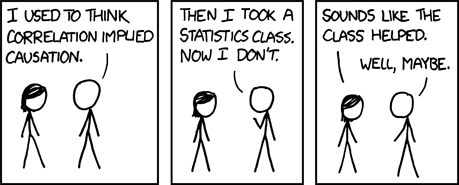
\includegraphics{images/xkcd/correlation-552.png}
    \caption{XKCD: Correlation, source \url{https://xkcd.com/552/}, used with permission.}
    \label{fig:xkcd-correlation}
\end{figure}

In terms of research hygiene, the research into the behaviours of Google Play Console and Android Vitals were debated and cross-checked with Google, and my paper~\citep{harty_google_play_console_insightful_development_using_android_vitals_and_pre_launch_reports} was reviewed by the Product Manager who was acknowledged with his permission in the paper.


\subsection{Discussion}~\label{case-study-kiwix-discussion}
\textit{(Explore what these outcomes mean for the use of analytics in mobile software more generally).}

Android Vitals is of limited value for low-volume apps as several reports are only available once there are data volumes to enable the data to be anonymized sufficiently to protect users' privacy. As the product owner confirmed at the time: \emph{``... it [information] only shows up for apps that have enough data to be privacy compliant"}~\footnote{unpublished correspondence with Google.}.

As reported in~\citep{harty_google_play_console_insightful_development_using_android_vitals_and_pre_launch_reports}, the Android Vitals reports were more relevant for apps with 10,000+ active users. Paradoxically, the threshold may be lower for apps which fail more often as they would generate more failure reports. However, actively testing this hypothesis may have adverse lifetime effects for the person who releases such poorly behaving apps, and knowingly doing so contravenes Google's policy for Google Play~\citep{google_play_developer_policy_center}~\footnote{The relevant section of the policy is currently available at:~\url{https://support.google.com/googleplay/android-developer/topic/9876964?hl=en&ref_topic=9858052,9857238,2856718,} and supported by training material at~\url{https://playacademy.exceedlms.com/student/path/65190-comply-with-google-play-s-spam-and-minimum-functionality-policies}}.


\textbf{MUST-DO} describe about the flaws discovered in GPC and Android Vitals and the discussions with Google Engineering.

\begin{comment}
Links to docs:
Android Developer Documentation: https://developer.android.com/topic/performance/vitals
Play Console Help Center: https://support.google.com/googleplay/android-developer/answer/7385505?hl=en-GB
Overview video: https://www.youtube.com/watch?v=vj3Y8L5HLdg

 https://android-developers.googleblog.com/2018/12/wrapping-up-for-2018-with-google-play.html, https://android-developers.googleblog.com/2017/07/android-vitals-increase-engagement-and.html and https://developer.android.com/topic/performance/vitals/ 
\end{comment}

\subsection{Summary of Kiwix Android Case Study}
% Joe's notes this is not compelling and doesn't compare with the other case studies.
% Why Kiwix, what did I gain, similarities and contrasts, why include in the PhD.

This is a long term study, where I was embedded as part of the development team for a period of the case study. We demonstrated it was practical to use only external, platform, analytics and still able to be effective in reducing the crash rate. For projects that do not use in-app crash reporting the platform tools are sufficient to make material improvements \emph{when the team actively monitors and addresses the crashes reported in the platform level analytics}. The practices need to be applied on a long term basis; with the loss of the project lead who focused on addressing the runtime failures the failure rates are increasing. Entropy increases.
% c.f. working with tech debt which has similar behaviours

%\akb{Include point about long term engagement needing tools like Vitals Scraper to provide data that can be used analyse performance of the app over time?}

The user interface of Google Play Console and Android Vitals was interactive and Google had removed an earlier feature where historic crashes could be downloaded for further analysis which meant the user interface was ephemeral, reports could not be stored easily (and even printing the reports as PDF files or on paper didn't capture the contents well) the user interface required human input and navigation, and retaining information for historical and trend analyses was difficult. Vitals Scraper was developed to address facilitate my ongoing research of this and other projects and enabled data, reports, crashes and ANRs to be recorded in ways that enabled comparisons and analysis. 

The case study was very useful in terms of providing  control and experiment apps. It was also the first of the experiments that set the scene and the direction for further case-studies.

The analytics reported on both \href{glossary_jvm}{JVM} and native crashes (written in C++) where that code is external and shared with various projects. 

% Provided materials published in various of my papers
This case study also led to the discovery of various flaws in Google Play Console and Android Vitals which led to the meetings, discussions and writing the report for the Google Engineering team. They have improved their product iteratively - v2 still had some flaws v3 has addressed some of these and similarly reduced some of the operability headaches.




%%%%%%%%%%%%%%%%%%%%%%%%%%%%%%%%%%%%%%%%%%%%%%%%%%%%%%%%%%%%%%%%%%%%%%%%
\par\noindent\rule{\textwidth}{0.4pt}
~\textbf{Earlier material follows}






% Following initial discussions about the crashes being reported in Android Vitals for version 2.5.0 of the Kiwix application, we collaborated on a week-long hackathon in Stockholm in August 2019. There, the developers ended up fixing some of the causes of the most frequent crashes with a surprisingly small amount of code of under 25 lines (including 10 lines of text added to the release log)\footnote{\url{https://github.com/kiwix/kiwix-android/pull/1388}}.



\subsection{Examples of real-time crashes}
Each of these examples exemplifies at least one characteristic of the reports that are provided by Android Vitals in Google Play.

\subsubsection{EsxRenderBucket::AddUnbucketedEntries(...)}
This crash is one of the most frequent crashes reported in early October 2020 and has been occurring on an ongoing basis according to Android Vitals for the current release of the Chemistry \& Physics simulations app (release 2020-04). Through analysis of the reports this crash only affects one release of the app (release 5200950) and it does not occur on the other three releases (6200950, 4200950, 3200950). It occurs on multiple manufacturer's device models, and on Android 9.0, 8.1, and 8.0). 

This crash is a native crash and mainly occurs within the context of \texttt{/system/app/Chrome/Chrome.apk} \textit{the web browser app created by Google!} The Kiwix apps rely on an embedded web browser, which is generally Google's Chrome browser, to render (\emph{i.e.} display) the content to the user\footnote{It also appears for other variants of the Android Chrome browser on some devices e.g. \texttt{/data/app/com.android.chrome-bAmCl9DcPfmqf3oKL54Efg==/base.apk (offset 0xbe7000)} and also the Android WebView component~\texttt{/data/app/com.google.android.webview-9ShSu\_81V02zu4ENrAjvJA==/lib/arm/libwebviewchromium.so} (also created by Google).}.

\begin{listing}[H]
\caption{Crash Cluster: EsxRenderBucket::AddUnbucketedEntries} \label{code:crash_cluster_add_unbucketed_entries}
\tiny
\begin{minted}{cpp}
*** *** *** *** *** *** *** *** *** *** *** *** *** *** *** ***
pid: 0, tid: 0 >>> org.kiwix.kiwixcustomphet <<<

backtrace:
  #00  pc 00000000001535a0  /vendor/lib/egl/libGLESv2_adreno.so (EsxRenderBucket::AddUnbucketedEntries(EsxCmdBufType, unsigned int)+132)
  #01  pc 0000000000152b17  /vendor/lib/egl/libGLESv2_adreno.so (EsxRenderBucket::BucketRenderingCmds(EsxRenderBucketParams*)+740)
  #02  pc 0000000000186a6d  /vendor/lib/egl/libGLESv2_adreno.so (EsxContext::BucketRenderingCmds(int)+712)
  #03  pc 00000000000e6987  /vendor/lib/egl/libGLESv2_adreno.so (EsxContext::BindDrawFramebuffer(EsxFramebufferObject*)+178)
  #04  pc 00000000000b6a5d  /vendor/lib/egl/libGLESv2_adreno.so (EsxContext::GlBindFramebuffer(unsigned int, unsigned int)+332)
  #05  pc 0000000001b8c659  /system/app/Chrome/Chrome.apk (offset 0x80c000)
\end{minted}

\end{listing}

Of the 53 crash clusters reported over the last 60 days for all Android versions and version 5200950 of the app, installed from Google Play, 16 of the 53 crash clusters are for this crash.

Searching local logs, generated using the opensource software~\texttt{vitals-scraper} that we created as part of this research we can see the same crash cluster has occurred in some, not all, of the Kiwix applications. The command used to find the files that contain this crash cluster is:~\texttt{grep -c EsxRenderBucket::AddUnbucketedEntries * | sort -t ':' -k 2 -g}. This returns a list of the files, sorted by the number of matches for the string found in each of the files. Here are the entries with at least one match.

\begin{listing}[H]
\caption{Logs that include crash cluster: EsxRenderBucket::AddUnbucketedEntries} \label{code:vitals_scraper_logs_add_unbucketed_entries}
\footnotesize
\begin{minted}{text}

android-crash-clusters-org.kiwix.kiwixcustomphet_1572958874833.json:2
android-crash-clusters-org.kiwix.kiwixmobile_1599898794048.json:2
phet-1-day-android-crash-clusters_1569599996989.json:2
android-crash-clusters-org.kiwix.kiwixcustomphet_1572966654935.json:3
android-crash-clusters-org.kiwix.kiwixmobile_1577913956806.json:3
android-crash-clusters-org.kiwix.kiwixcustomphet_1574380641173.json:4
android-crash-clusters-org.kiwix.kiwixcustomphet_1572976000060.json:5
android-crash-clusters-org.kiwix.kiwixcustomphet_1577913523667.json:5
android-crash-clusters-org.kiwix.kiwixcustomphet_1601883786819.json:5
wikimed-60-days-android-crash-clusters_1568705009571.json:6
phet-7-days-android-crash-clusters_1569484818005.json:13
android-crash-clusters-org.kiwix.kiwixcustomphet_1573403158401.json:14
android-crash-clusters-org.kiwix.kiwixcustomphet_1599898464809.json:14
phet-60-days-android-crash-clusters_1568703927627.json:18
android-crash-clusters-org.kiwix.kiwixcustomphet_1572903426940.json:21
phet-60-days-android-crash-clusters_1565933377493.json:21
android-crash-clusters-org.kiwix.kiwixcustomphet_1572812538185.json:25
\end{minted}

\end{listing}

From these results the crash occurs most often in the Physics \& Chemistry simulation custom app (these include the phrase `phet'\footnote{`phet' is the term used for the source of the contents used in this custom app, i.e. the source of the various Chemistry and Physics simulations, written in HTML5. They are extremely rich in terms of their content and dynamic rendering as they provide interactive, dynamic simulations.} as part of the filename. It also occurred relatively infrequently in two other of the apps: five times in the core Kiwix app, and six times in the Wikipedia in English app. The core Kiwix app can be used with the same contents as the project bundles in the custom apps, so some of the crashes~\emph{might} be for the same content, we don't know enough from the stack trace to determine the contents. the reasons for the error in the custom WikiMed app are not known at this stage. 

Searching online, using Google Search, for \texttt{EsxRenderBucket::AddUnbucketedEntries} finds a similar stack trace occurs with the Unity SDK and it appears to be related to a particular chipset:
\begin{itemize}
    \item \href{https://developer.qualcomm.com/forum/qdn-forums/software/adreno-gpu-sdk/67924}{Forums - Help with crash in {\footnotesize libGLESv2\_adreno.so (EsxRenderBucket::AddUnbucketedEntries)}} 2020
    % \item \href{https://github.com/flutter/flutter/issues/38676}{/system/vendor/lib/egl/libGLESv2_adreno.so #38676} 2019
    % \item \href{https://stackoverflow.com/questions/29728931/libglesv2-adreno-so-game-crash-in-galaxy-note-4-and-lollipop-5-0}{libGLESv2_adreno.so game crash in Galaxy Note 4 and Lollipop 5.0} 2015
    \item \href{https://forum.unity.com/threads/unity-2019-android-build-crashes-on-devices-using-adreno-506-gpu.712229/}{Unity 2019 Android build crashes on devices using Adreno 506 GPU}. This bug report includes several different method names where the crash occurs. Various developers report the issue, \href{https://forum.unity.com/members/waldgeist.1371619/}{Waldgeist} reporting the one with this method name.
\end{itemize}

The bug appears hard for developers to reproduce and from the app developer's perspective it happens in software they cannot fix themselves. 

As Ogien reports in~\href{https://forum.unity.com/threads/unity-2017-2-crashes-vs-5-6-2f1.511995/}{Unity 2017.2 Crashes vs 5.6.2f1} they may be able to identify correlations (in this example using a screenshot from Android Vitals, I believe, as shown in Figure~\ref{fig:unity-2017-2-android-vitals-annotated-graph}). The Unity support team state the bug may have been fixed and the developer promised to try the new release and report back at the time, in 2018, however they have not done so online at least\footnote{This user was online more recently, including \nth{24} September 2020.} so that issue has an indeterminate result from a research perspective.

\begin{figure}[htbp!]
    \centering
    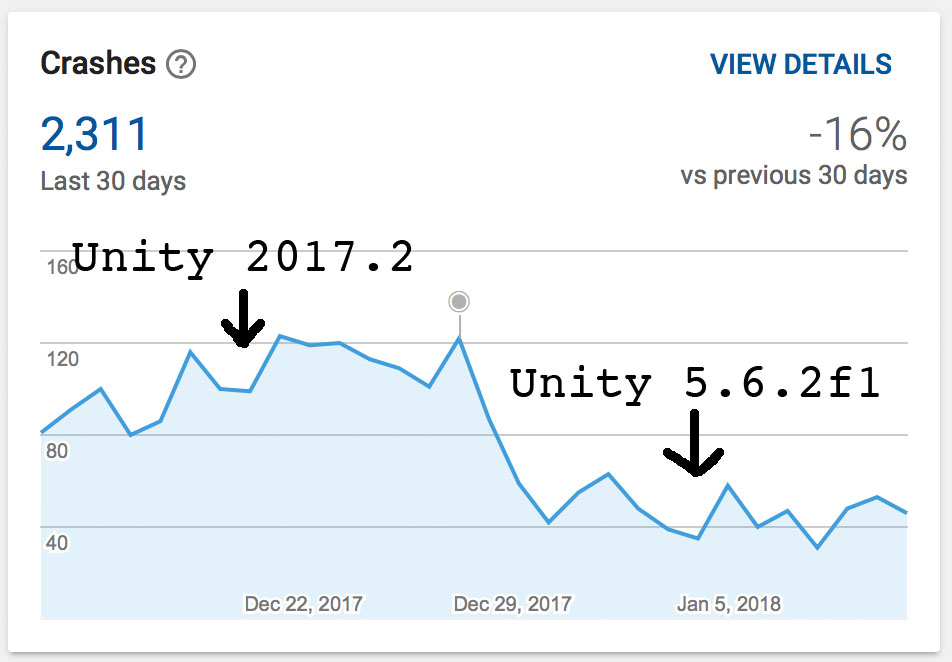
\includegraphics[width=12cm]{images/unity-forum/unity-2017-2-android-vitals.jpg}
    \caption{Unity 2017.2 Android-Vitals annotated graph (\url{https://forum.unity.com/threads/unity-2017-2-crashes-vs-5-6-2f1.511995/}}
    \label{fig:unity-2017-2-android-vitals-annotated-graph}
\end{figure}


\subsubsection{Android App Bundling}~\label{kiwix-android-app-bundling-crashes}
MUST-DO complete this section

MUST-DO Discuss the augmented crash stack trace utility, how it works, and why we did~\emph{not} use it in Google Play apps.


\subsection{Lessons learned from this case study}

As~\citep{kidwell2015_toward_fault_taxonomy_application_of_software_analytics} notes, previous research by~\citep{weider1998_software_fault_prevention_in_coding_and_RCA} nearly half the faults were introduced during coding and \emph{``...many of the faults were preventable"}. These results were borne out in the Kiwix Android case study where some of the most frequent crashes were null pointer errors in the Java code. For the Kiwix Android project one of the longer term challenges was the youth of many of the volunteer contributors including some of the development leads who were often teenagers and pre-undergraduate level software developers who wouldn't have the expertise expected of professional software developers\footnote{(They often joined via Google Code-in~\citep{google_code_in_archive} or Google Summer of Code~\citep{google_summer_of_code}).}. While there may well be training techniques and software tools, including Android Lint, that may have been able to find some of the causes of the crashes reported by Android Vitals it's unlikely that these volunteers would choose to use those tools or want to undergo training. And as interviews with developers demonstrated the perceived effort of dealing with static analysis reports and the volume of false positives mean developers don't use static analysis tools very often to find bugs~\citep{johnson2013_why_dont_devs_use_static_analysis}.

%\subsection{Summary of Kiwix Android Case Study}
\subsection{Overall evaluation of the Kiwix case study}
Within five months the project was able to reduce the crash rate of the core application from over 3\% to around a tenth of that figure. One of the main causes was the focus on addressing the most prevalently reported crash clusters in Android Vitals. This was not the only cause of the improvement, the software was also being revised and updated, this included replacing some of the existing Java code with Kotlin equivalents. 

Empirical research in Android apps that migrate from Java to Kotlin indicate the code quality often improves in tandem according to static analysis of the binary files of various releases of the studied opensource apps~\cite{GoisMateus2019_an_empirical_study_on_the_quality_of_android_apps_in_kotlin}. That work does not investigate exceptions or crashes, it does include the Kiwix Android project~\footnote{Kiwix is listed as one of the projects their research investigated:~\url{https://github.com/UPHF/kotlinandroid/blob/master/docs/fdroid_all.md}.}. However, their research predates both my case study and when the Kiwix codebase transitioned to Kotlin.

The Kiwix Android project team continued to file bug reports and address them, for instance {\small~\href{https://github.com/kiwix/kiwix-android/issues/2104}{\texttt{github.com/kiwix/kiwix-android/issues/2104}}} 
provides an example of the lead developer raising a bug report for a crash reported by Android Vitals; and \\{\small ~\href{https://github.com/kiwix/kiwix-android/issues?q=is\%3Aissue+\%22crash+report\%22+}{\texttt{github.com/kiwix/kiwix-android/issues?q=is\%3Aissue+\%22crash+report\%22+}}} provides an up-to-date view of issues labeled with ``crash report". 

In conclusion, addressing crash reports was performed actively by the developers and the crash rate of all the updated Android apps updated since the start of the case study did improve. However, following the loss of the (professional) lead developer the crash rate of the flagship app has increased, and may not decrease unless the project team take ownership of addressing the causes of the increased crash rate.

%%%%%%%%%%%%%%%%%%%%%%%%%%%%%%%%%%
\par\noindent\rule{\textwidth}{0.4pt}
%%%%%%%%%%%%%%%%%%%%%%%%%%%%%%%%%%

Confounding factors, in the discussion chapter. e.g. the observations of the crash rate increasing, the change of lead developer. Gains are not permanent, and need active engagement. c.f. more recent Kiwix data shows... ditto Catrobat.

